% load packages
\documentclass{article}
\usepackage[english]{babel}
\usepackage[utf8]{inputenc}
\usepackage{johd}

\title{Forecasting Air Cargo Demand for Southeast Asia}

\author{Josephine Tan Xin Yi$^{a}$, Michael Hoon Yong Hau$^{a}$\\
        \small $^{a}$Singapore University of Technology and Design, Singapore \\\\
        \small \textbf{Principal Investigator}: Peter Jackson$^{b}$, \textbf{Project Lead}: Jamie Bloomfield$^{b}$ \\
        \small $^{b}$Aviation Studies Institute, Singapore University of Technology and Design, Singapore \\
}

\date{$5\textsuperscript{th}$ December $2022$} %leave blank

\begin{document}

\maketitle

\begin{figure}[t!]
    \centering
    
\includegraphics[width=0.2\textwidth]{images/ASI Graphics/sutd-asi-logo-web-2021-fc.png}
    
\includegraphics[width=0.2\textwidth]{images/ASI Graphics/asi-logo-web-2022-fc.png}
    
\includegraphics[width=0.2\textwidth]{images/ASI Graphics/asi-logo-web-2021-fc-02-v2.png}
    \label{titlefig}
\end{figure}

\begin{abstract} 
\noindent A short (up to 250 words) summary of the main contributions of the paper and the context of the research. Full length papers discuss and illustrate methods, challenges, and limitations in the creation, collection, management, access, processing, or analysis of data in humanities research, including standards and formats. These aspects must not necessarily be discussed with reference to a specific dataset (or collection thereof) but, if your paper focusses on particular datasets, we advise to add the dataset metadata under the section ‘Dataset description’. This template provides a general outline for full length papers and authors can adapt the headings and include subheadings as they find appropriate. Please delete or replace the blue text with your own text in black.  
\end{abstract}

\noindent\keywords{Air Freight Demand; Air Cargo; Forecasting}

\newpage

\tableofcontents

\newpage

\section{Introduction}

\subsection{Objective}

This project is performed under SUTD’s Undergraduate Research Opportunities Programme (UROP), supervised through the Aviation Studies Institute (ASI). This provides university students with the opportunity to apply research techniques as part of their undergraduate studies for short duration projects (up to c. 3-months). \\

\noindent The project objective is to support the prediction of future air cargo demand within Asia by identifying the factors of significance and reliable data sources, whilst leveraging confidential historical air cargo demand data supplied by a collaborating organisation (International Air Transport Association, [IATA]). \\

\noindent This involves (and is dependent upon) working with commercial data supplied by the commercial partner, in addition to open source data. The work would be the first step in developing applied insights of direct relevance to the air transport industry. \\

\noindent A key aspect of the work involves assessing which datasets are both relevant and reliable to be of use on a repeat basis.

\subsection{Motivation}

Air Cargo has grown in relevance during the COVID-19 pandemic as a means to transport perishable goods in a timely manner. Despite extensive data on historical cargo demand, predicting future demand remains poorly defined. Whilst there is a general correlation with the Gross Domestic Product (GDP), several other macroeconomic factors also play a pivotal role in different geographical regions. \\

\noindent This project involves identifying the factors of significance to air cargo demand which can be used to predict future air cargo demand within the Southeast Asia region over the long-time horizons. \\

\noindent The work will use extensive historical data related to cargo demand (obtained from the IATA CargoIS platform), open-source macroeconomic data (historical and forecast) and data models that will search for correlations. \\

\noindent A second challenge will be to develop mathematical models that search for correlations between the acceptable data and the historical air cargo demand. These will be used to identify the factors of significance for use in predicting future air cargo demand in the region. 


\section{Analysis of Cargo Data}

After obtaining the relevant cargo dataset from IATA in CSV format, DBeaver was used as a relational database management system (RDBMS) to manage the provided data. SQLite was used as our main language to query the required data. \\

\noindent The initial dataset provided by IATA's CargoIS platform ranged monthly from January 2015 to December 2018, and included each origin country's weight and number of shipments to the receiving country.


\subsection{Data Cleaning and Management}

As the scope of our project involves analysis of air cargo demand within Asia, we have decided to focus on analysis between ASEAN countries within the Southeast Asia region. This significantly narrows down and reduces the size of the dataset, in hopes of easier identification of relevant correlations with macroeconomic data. \\

\noindent One of our initial challenges while working with the data was that the different countries had naturally vastly different number of shipments and weights, by virtue of their economic status. This resulted in a relatively high sample standard deviation across the ASEAN region, which made it difficult to obtain useful data analysis on the raw data. As a result, we decided to employ feature scaling techniques on the raw data, namely base 10 logarithmic scaling, to better visualise the data on our map and radar plots. \\

\noindent Prior to obtaining the CargoIS data from IATA, we had sourced for and collated a multitude of macroeconomic and non-macroeconomic datasets for each country on an annual basis, as we were expecting to aggregate the given data annually and forecast beyond 2022. \\

\noindent After obtaining the CargoIS data however, we had realised that it ranges only from 2015 to 2018, which would mean only four available data points if we were to aggregate the data yearly for analysis. This would be insufficient data for any meaningful analysis as the results would not be credible, due to a low sample size. Following this, we decided to aggregate each year's worth of data into quarters, as sourcing for reliable yet open-source macroeconomic data on a monthly basis proved to be a significant challenge. This would bring us to a total of 16 data points per country, which is enough to show any potential trends and seasonality in the data. 

\subsection{Exploratory Data Analysis}

\subsubsection{Air Cargo Trade Relations}

Initial analysis was performed using \textit{R} code in \textit{RStudio} to visualise the key geographical flows and movements of air freight between ASEAN countries. This was done by combining our current dataset with open source Geospatial data from Google\footnote{Google Dataset Publishing Language, \url{https://github.com/google/dspl}}, which contained the longitude and latitude coordinates of each country. Due to limitations of the dataset, this geospatial plot does not represent the exact takeoff and landing coordinates of each flight, nor of the flight path taken by each plane. \\ 

\noindent Shipment activity of all ASEAN states aggregated from 2015 to 2018 are shown below, with the thickness of each line indicating the relative number of exports from each country.

\begin{figure}[H]
    \centering
    \subfloat[\centering Singapore's Aggregated Exports]{{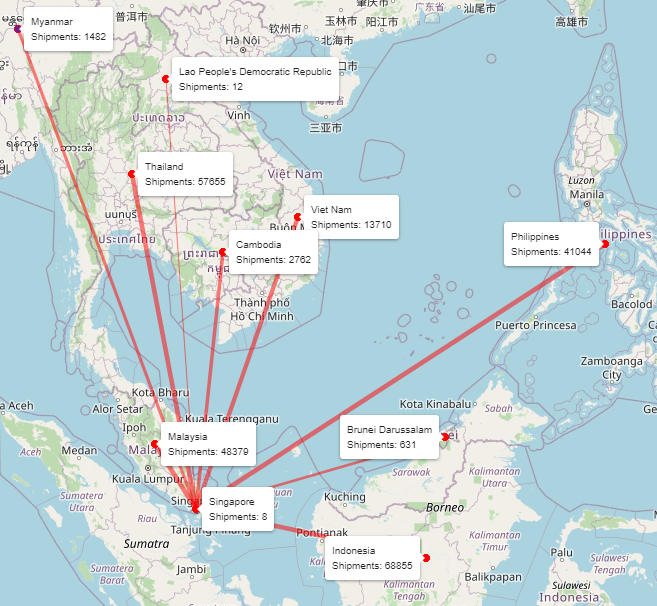
\includegraphics[width=0.475\textwidth]{images/Map Visualisations/Singapore_Exports.png}}}
    \qquad
    \subfloat[\centering Malaysia's Aggregated Exports]{{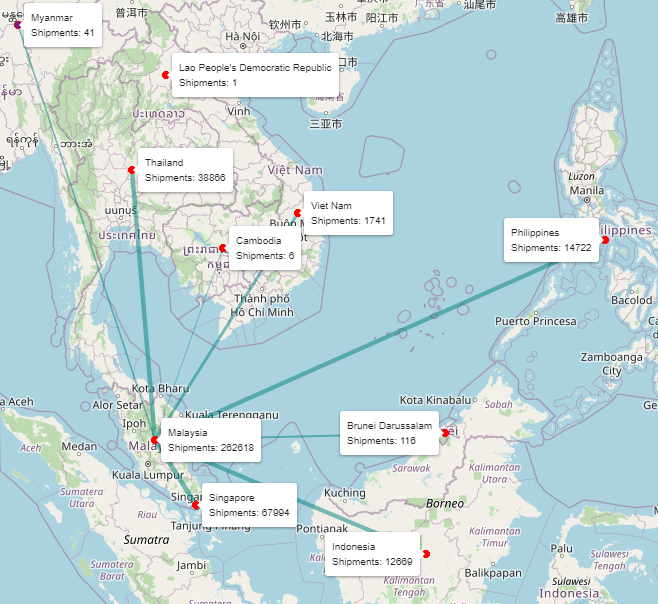
\includegraphics[width=0.475\textwidth]{images/Map Visualisations/Malaysia_Exports.png}}}
    \caption{Singapore and Malaysia}
    \label{fig: sg}
\end{figure}

\begin{figure}[H]
    \centering
    \subfloat[\centering Thailand's Aggregated Exports]{{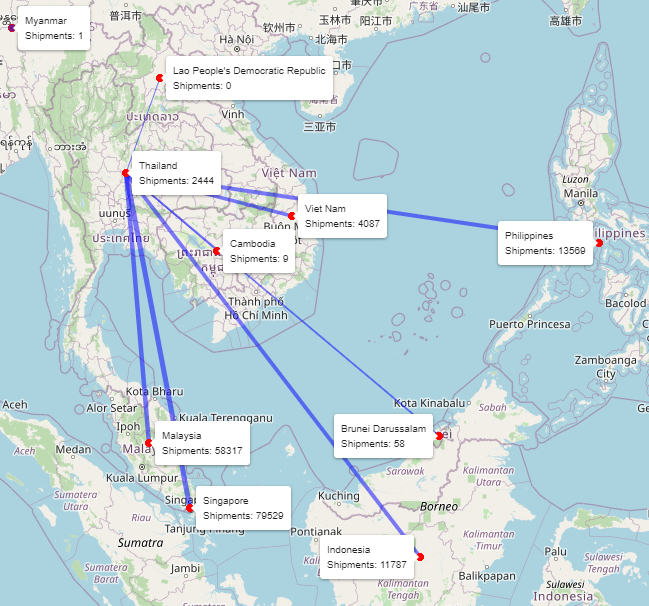
\includegraphics[width=0.475\textwidth]{images/Map Visualisations/Thailand_Exports.png}}}
    \qquad
    \subfloat[\centering Vietnam's Aggregated Exports]{{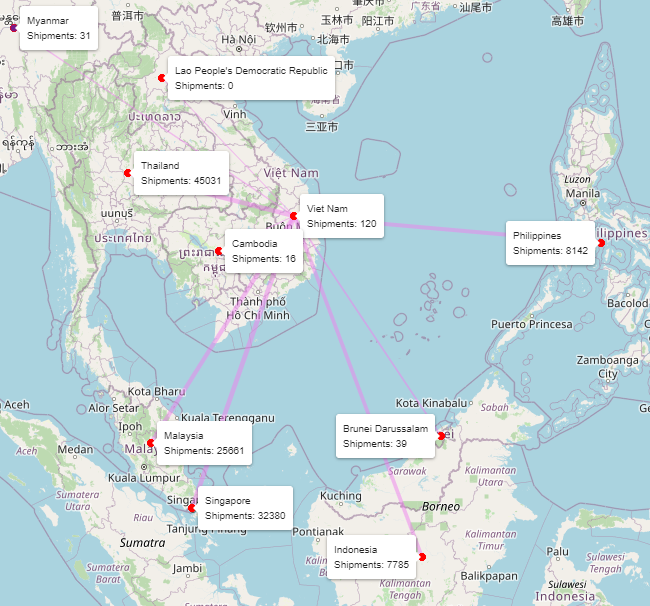
\includegraphics[width=0.475\textwidth]{images/Map Visualisations/Vietnam_Exports.png}}}
    \caption{Thailand and Vietnam}
    \label{fig: sg}
\end{figure}

\begin{figure}[H]
    \centering
    \subfloat[\centering Philippines's Aggregated Exports]{{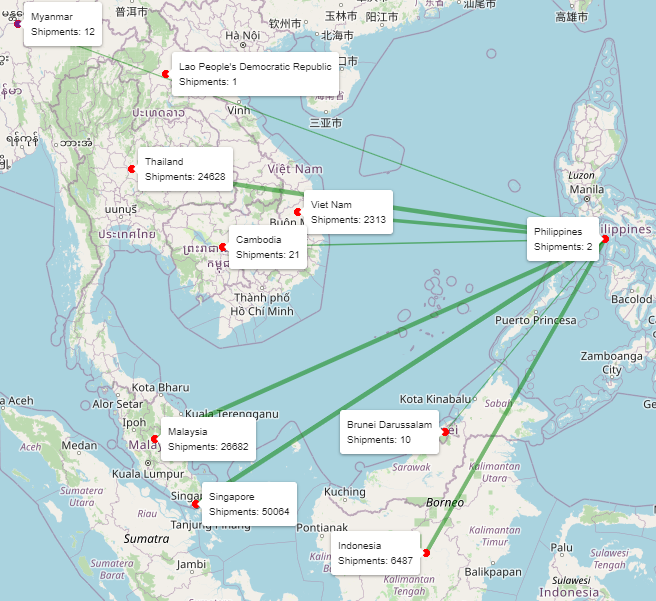
\includegraphics[width=0.475\textwidth]{images/Map Visualisations/Philippines_Exports.png}}}
    \qquad
    \subfloat[\centering Brunei's Aggregated Exports]{{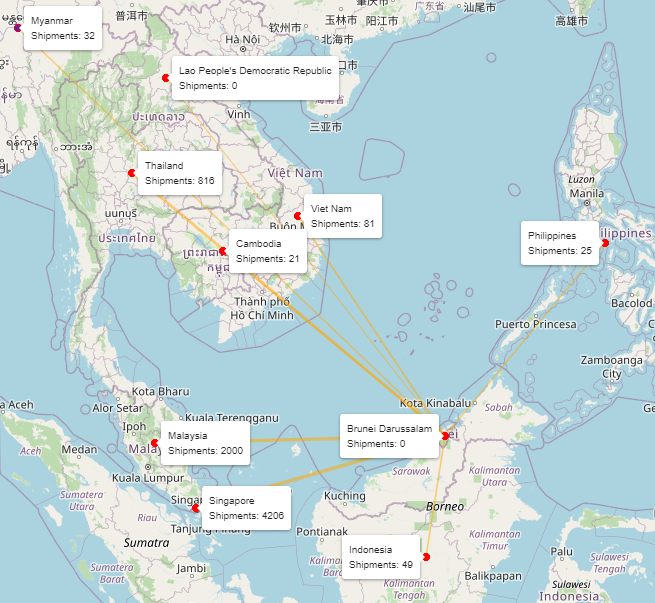
\includegraphics[width=0.475\textwidth]{images/Map Visualisations/Brunei_Exports.png}}}
    \caption{Philippines and Brunei}
    \label{fig: sg}
\end{figure}

\begin{figure}[H]
    \centering
    \subfloat[\centering Cambodia's Aggregated Exports]{{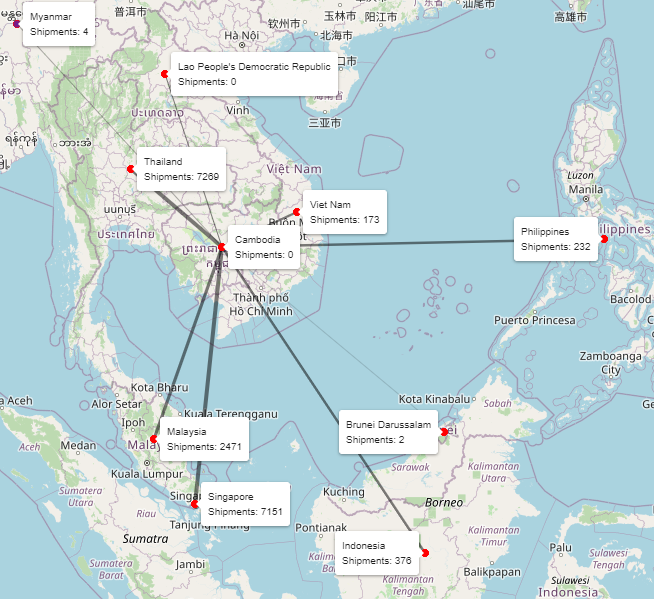
\includegraphics[width=0.475\textwidth]{images/Map Visualisations/Cambodia_Exports.png}}}
    \qquad
    \subfloat[\centering Laos' Aggregated Exports]{{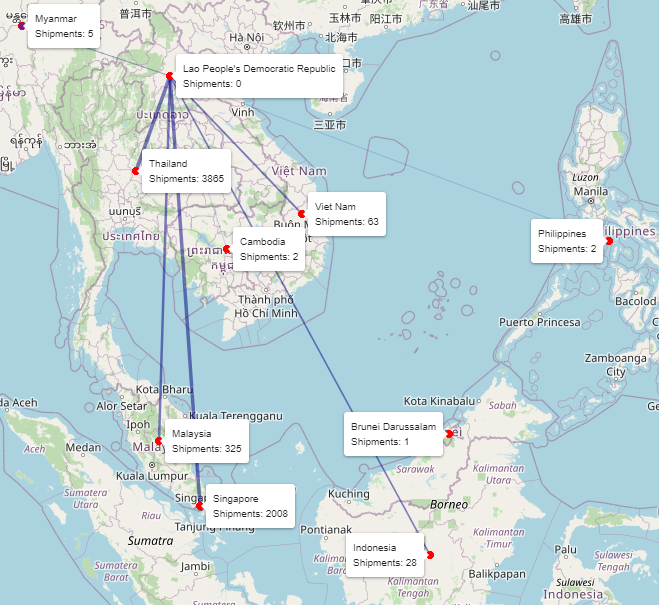
\includegraphics[width=0.475\textwidth]{images/Map Visualisations/Laos_Exports.png}}}
    \caption{Cambodia and Laos}
    \label{fig: sg}
\end{figure}

\begin{figure}[H]
    \centering
    \subfloat[\centering Indonesia's Aggregated Exports]{{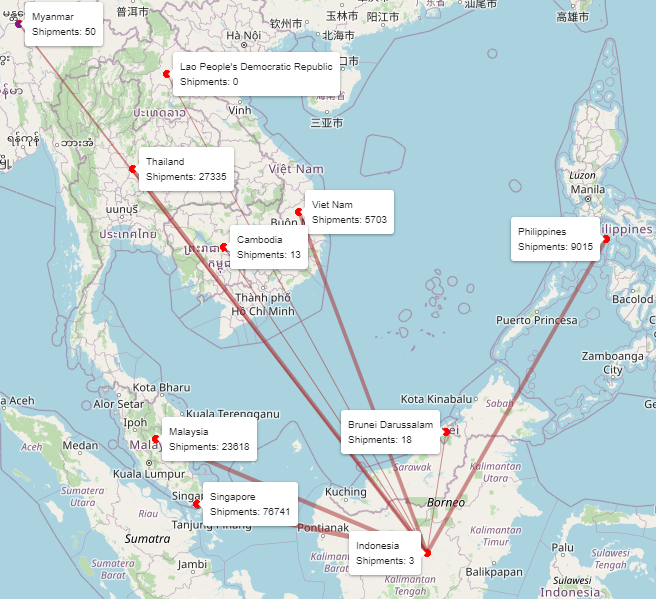
\includegraphics[width=0.475\textwidth]{images/Map Visualisations/Indonesia_Exports.png}}}
    \qquad
    \subfloat[\centering Myanmar's Aggregated Exports]{{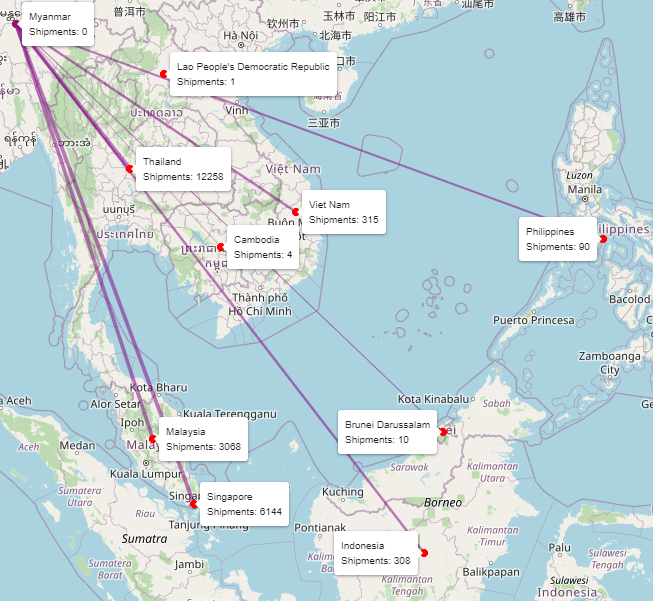
\includegraphics[width=0.475\textwidth]{images/Map Visualisations/Myanmar_Exports.png}}}
    \caption{Indonesia and Myanmar}
    \label{fig: sg}
\end{figure}

\noindent Some key conclusions can be identified from the geospatial data: \\

\begin{itemize}
    \item Lao PDR has one of the lowest cargo activity amongst all the ASEAN countries. Despite exporting to many countries, it does not seem to correspondingly receive the same amount of imports (Interestingly, Laos is the only land-locked country in Southeast Asia). 
    \item Different countries have different major shipment partners, although Singapore, Malaysia, and Thailand have particularly high proportions of shipment activity with other countries regardless.
    \item Malaysia has a disproportionately large shipment activity with itself compared to other countries, although where exactly within itself is not specified due to the lack of data.
\end{itemize}

\newpage

\subsubsection{Annual Imports of Air Cargo Per Country}

Interactive radar charts were also generated in \textit{Python} code, with options to display the years as coloured overlay. The radar charts give a better overview on the interaction between the ASEAN countries, which in this case represents the total number of imports per year. The number of shipments have been log-scaled, and as such the axis represents the scaled value of shipments, i.e. number of shipments $= 10^r$, with $r$ being the value on the axis. \\

\noindent We are also able to visualise and compare each country's internal shipments with that of neighbouring countries, as well as countries with no interaction between one another. 

\begin{figure}[H]
    \centering
    \subfloat[\centering Singapore's Annual Imports]{{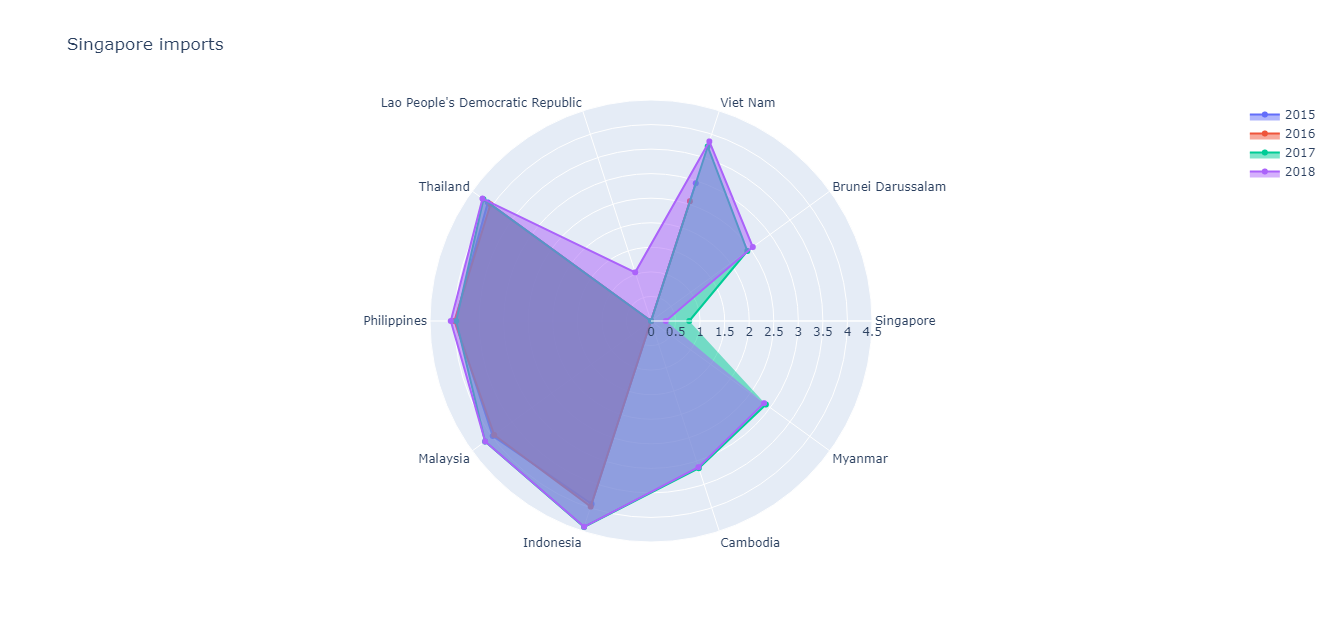
\includegraphics[width=0.475\textwidth]{images/Radar Plots/Singapore_Radar.png}}}
    \qquad
    \subfloat[\centering Malaysia's Annual Imports]{{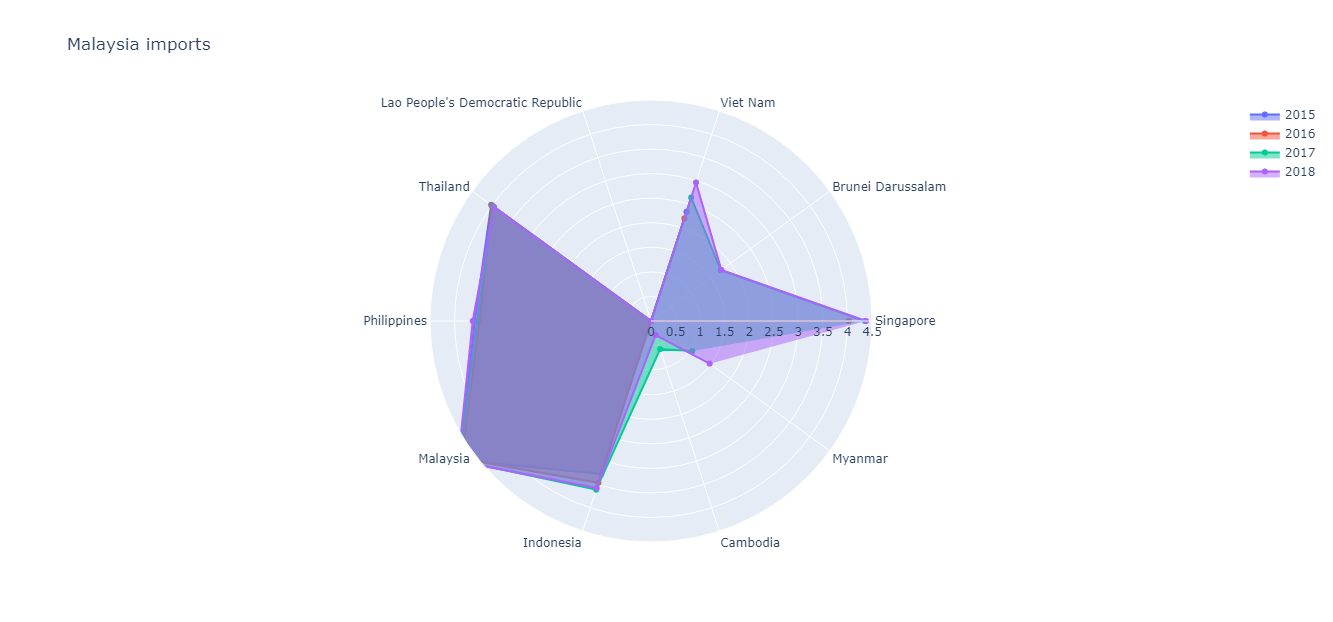
\includegraphics[width=0.475\textwidth]{images/Radar Plots/Malaysia_Radar.png}}}
    \caption{Singapore and Malaysia}
    \label{fig: sm}
\end{figure}

\begin{figure}[H]
    \centering
    \subfloat[\centering Thailand's Annual Imports]{{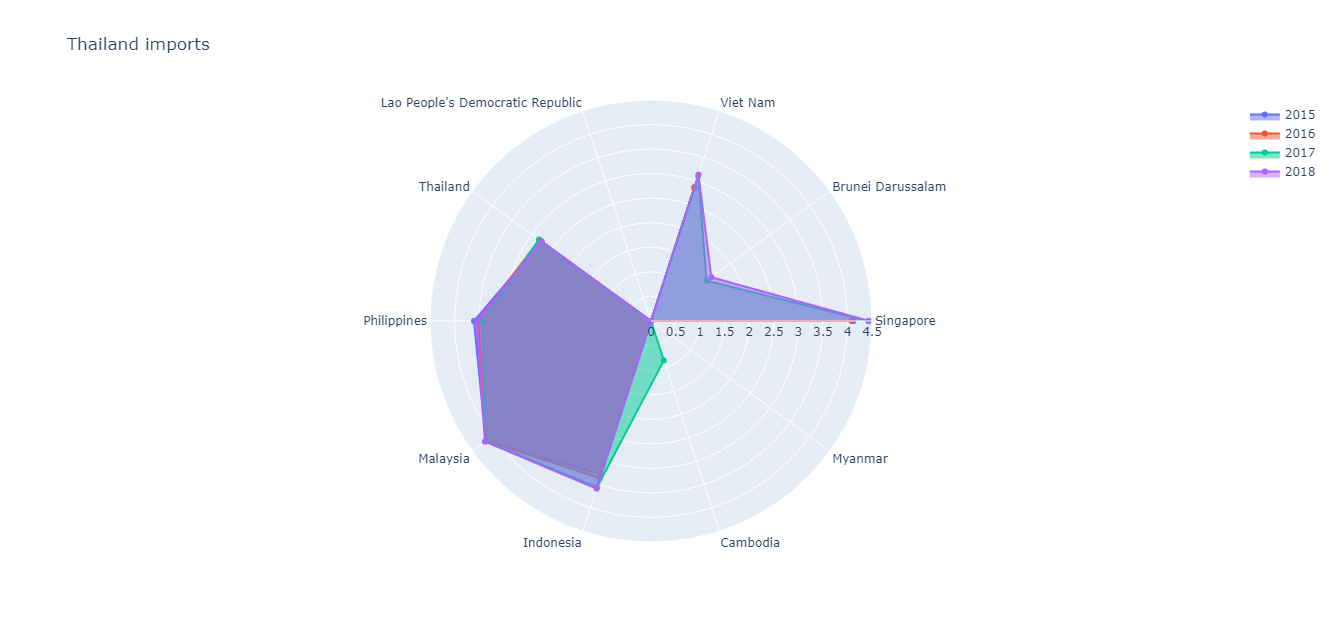
\includegraphics[width=0.475\textwidth]{images/Radar Plots/Thailand_Radar.png}}}
    \qquad
    \subfloat[\centering Vietnam's Annual Imports]{{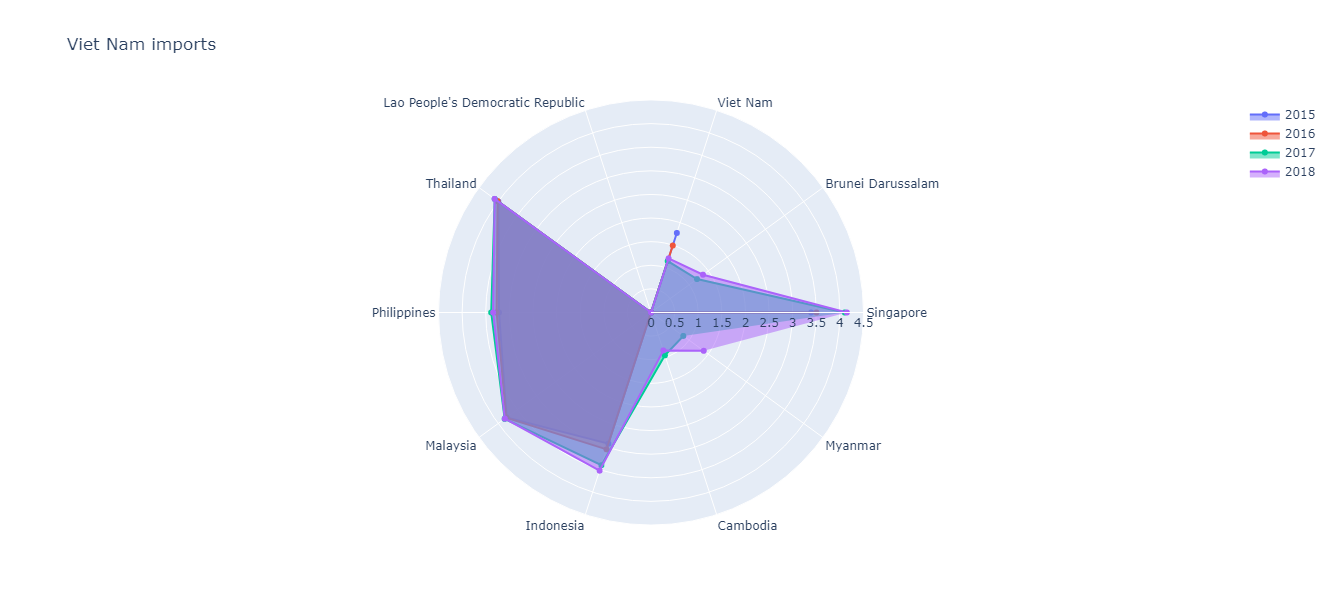
\includegraphics[width=0.475\textwidth]{images/Radar Plots/Vietnam_Radar.png}}}
    \caption{Thailand and Vietnam}
    \label{fig: tv}
\end{figure}

\begin{figure}[H]
    \centering
    \subfloat[\centering Philippines's Annual Imports]{{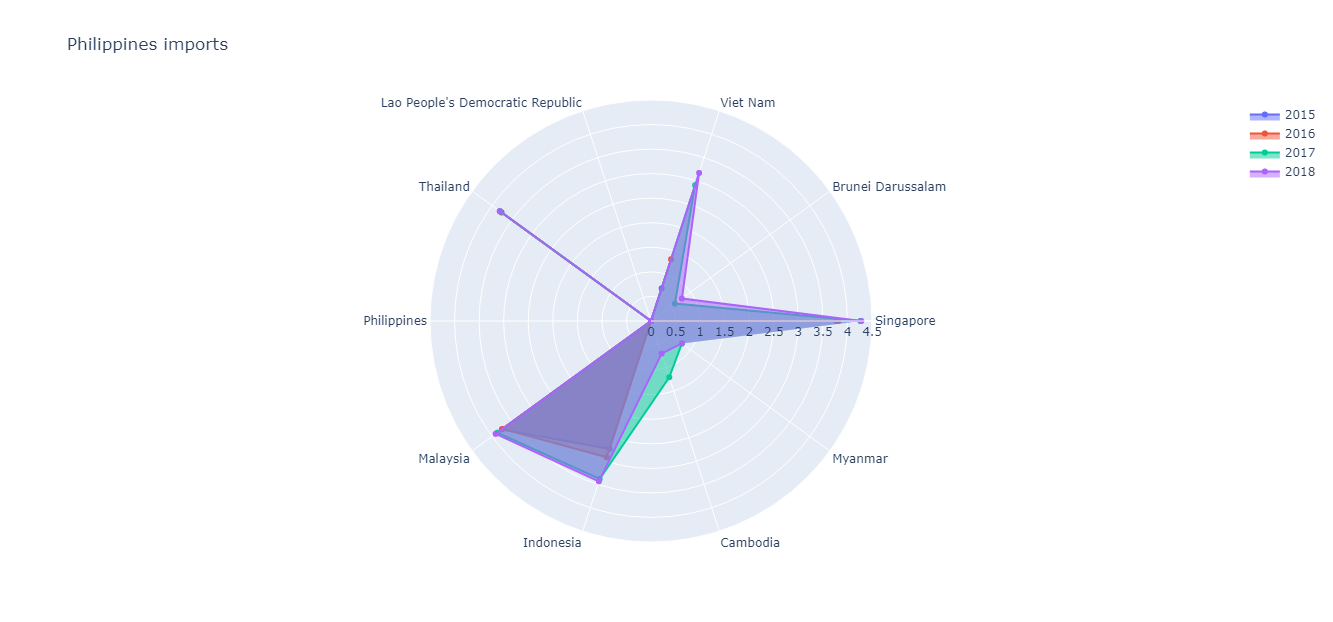
\includegraphics[width=0.475\textwidth]{images/Radar Plots/Philippines_Radar.png}}}
    \qquad
    \subfloat[\centering Brunei's Annual Imports]{{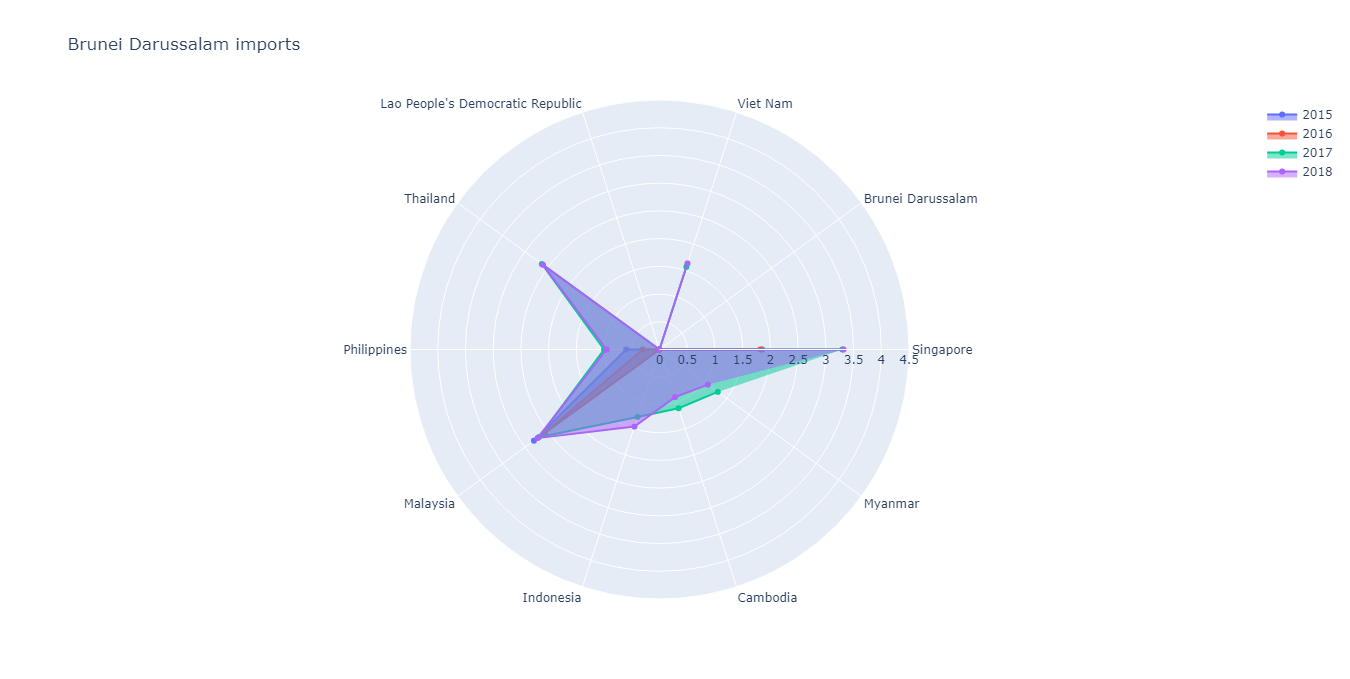
\includegraphics[width=0.475\textwidth]{images/Radar Plots/Brunei_Radar.png}}}
    \caption{Philippines and Brunei}
    \label{fig: pb}
\end{figure}

\begin{figure}[H]
    \centering
    \subfloat[\centering Cambodia's Annual Imports]{{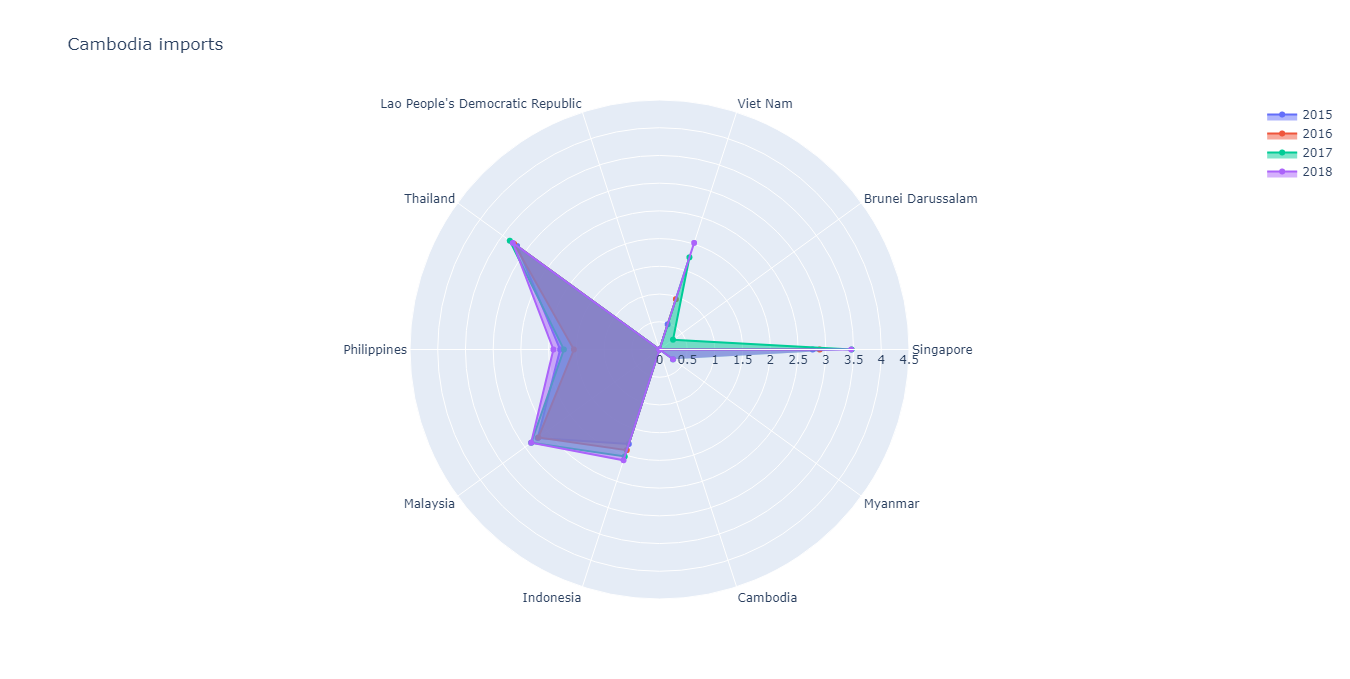
\includegraphics[width=0.475\textwidth]{images/Radar Plots/Cambodia_Radar.png}}}
    \qquad
    \subfloat[\centering Laos' Annual Imports]{{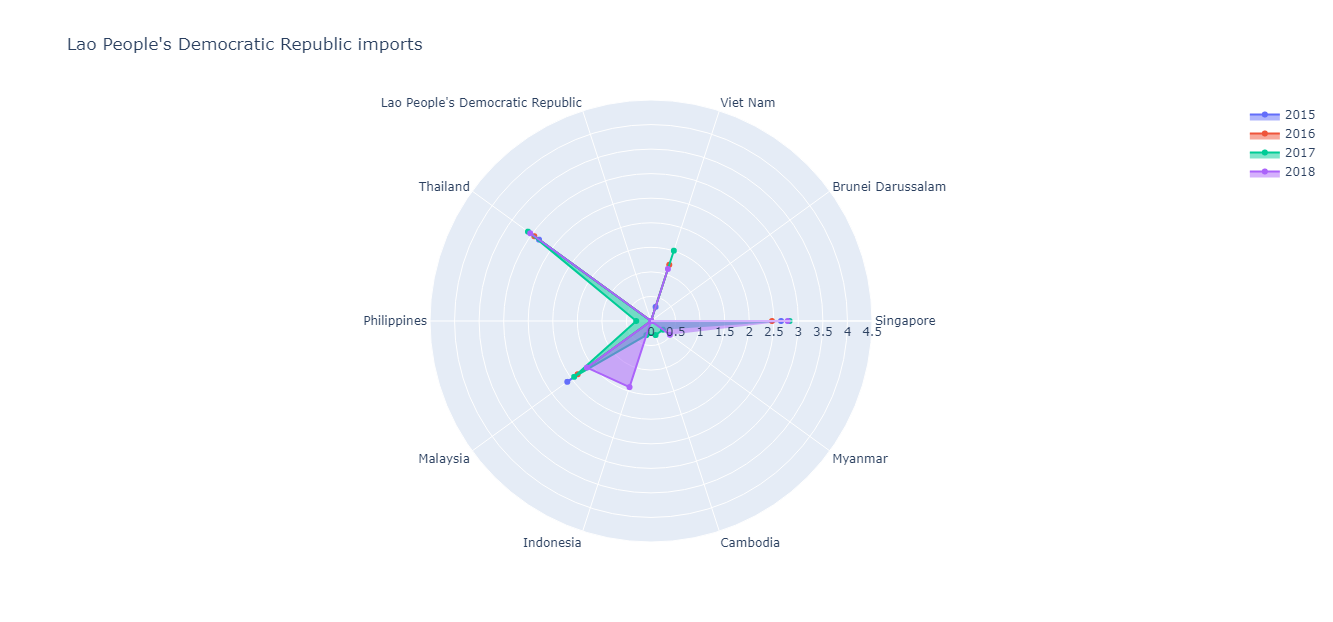
\includegraphics[width=0.475\textwidth]{images/Radar Plots/Lao_Radar.png}}}
    \caption{Cambodia and Laos}
    \label{fig: cl}
\end{figure}

\begin{figure}[H]
    \centering
    \subfloat[\centering Indonesia's Annual Imports]{{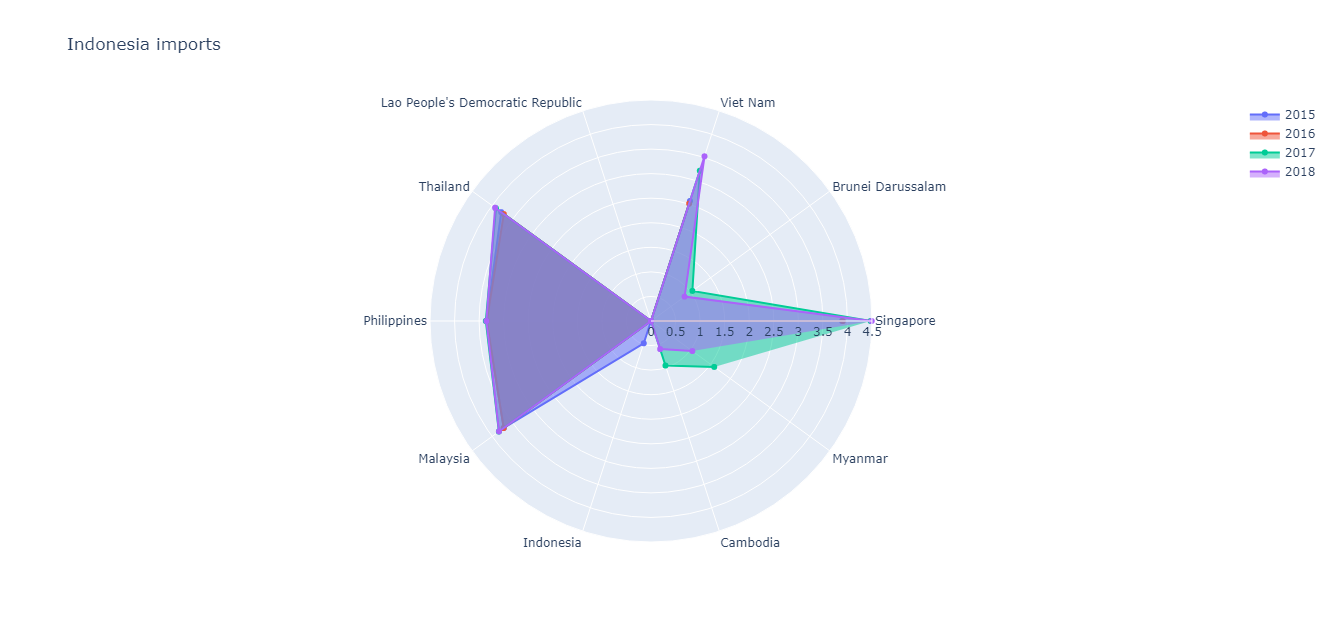
\includegraphics[width=0.475\textwidth]{images/Radar Plots/Indonesia_Radar.png}}}
    \qquad
    \subfloat[\centering Myanmar's Annual Imports]{{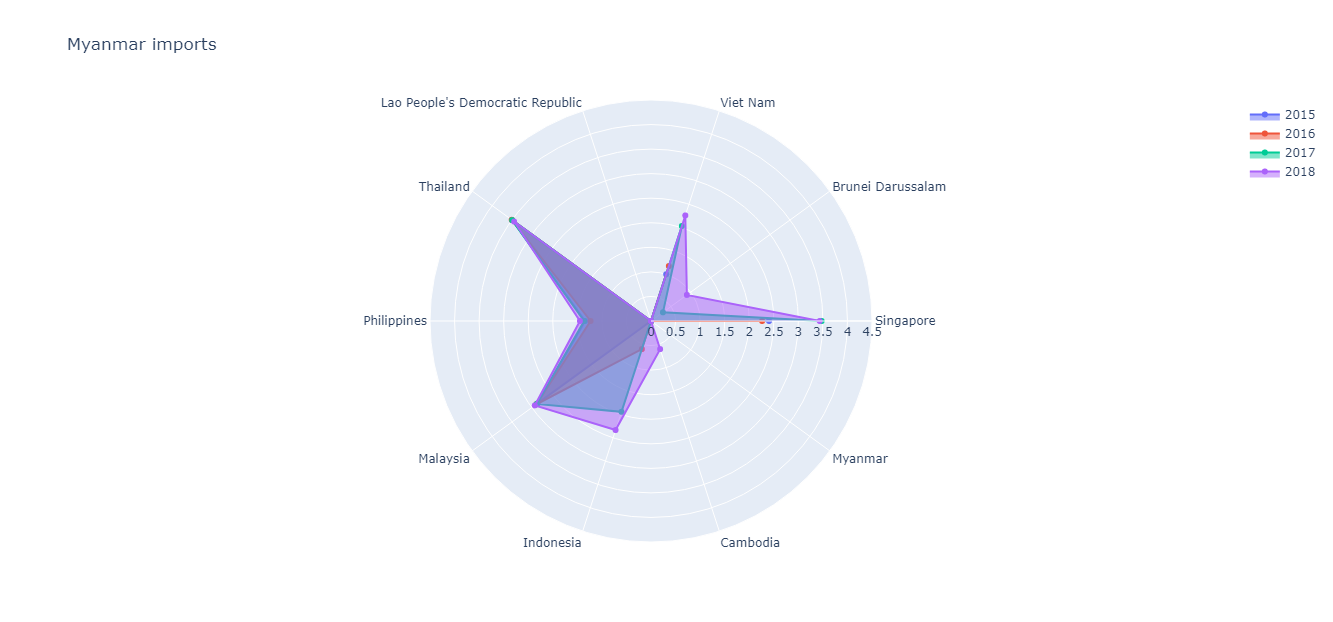
\includegraphics[width=0.475\textwidth]{images/Radar Plots/Myanmar_Radar.png}}}
    \caption{Indonesia and Myanmar}
    \label{fig: im}
\end{figure} 

\noindent Some interesting analysis to note: \\

\begin{itemize}
    \item While most countries do not import from themselves, Malaysia seems to once again have a disproportionately high internal imports to itself. 
    \item There seems to be a noticeable jump in the number of imports from 2016 to 2017, which is consistent for all countries. The number of imports from 2015 to 2016 and 2017 to 2018 stays relatively consistent, however.
    \item The disproportionate increase in trade between countries from 2016 to 2017 might be due to more countries participating in the ASEAN Free Trade Area (AFTA). The objectives of the AFTA include the elimination and reduction of import duties, removal of Non-Tariff Barriers (NTBs), among many others, aimed at creating a robust intra-ASEAN trade.
\end{itemize}

\newpage

\subsubsection{Quarterly Air Freight Demand}
The following figures depict line charts, displaying the number of shipment activity (total imports and exports) for each country within the ASEAN region. The plots are separated into two, with one including the countries with higher shipment activity, and the other with lower shipment activity. This allows for better visual comparison between countries with vastly differing shipment activity. 

\begin{figure}[H]
\centering
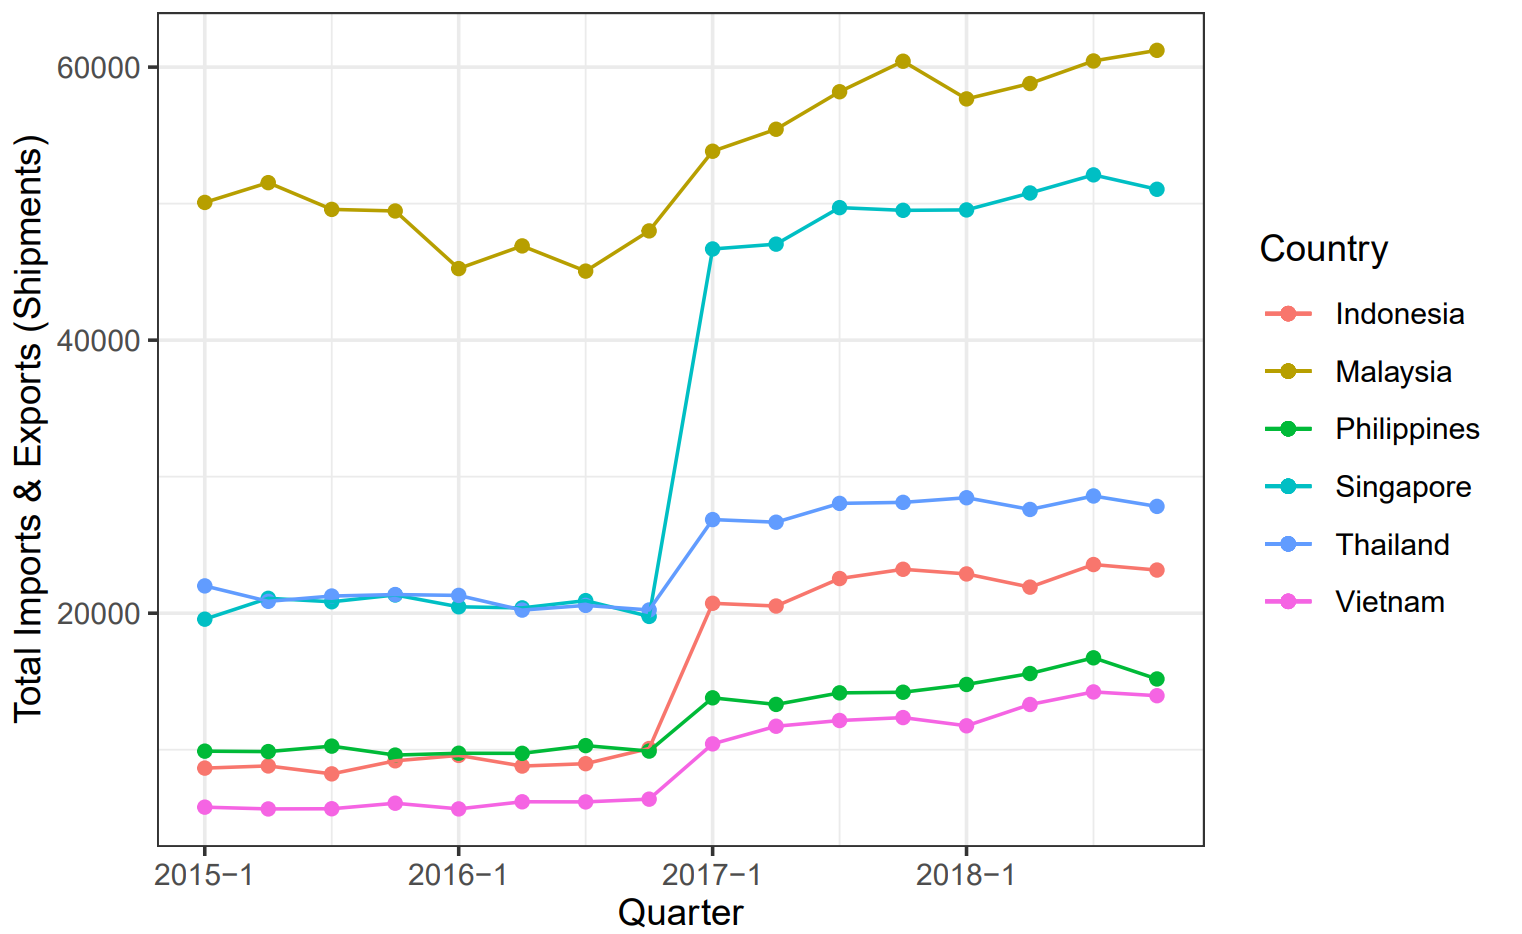
\includegraphics[width=1\textwidth]{images/Line Plots/ASEAN/ASEAN_Large_Quarterly_Shipments_BigFont.png}
\caption{\label{fig2}Total Shipments for Larger Activity Countries}
\end{figure}

\begin{figure}[H]
\centering
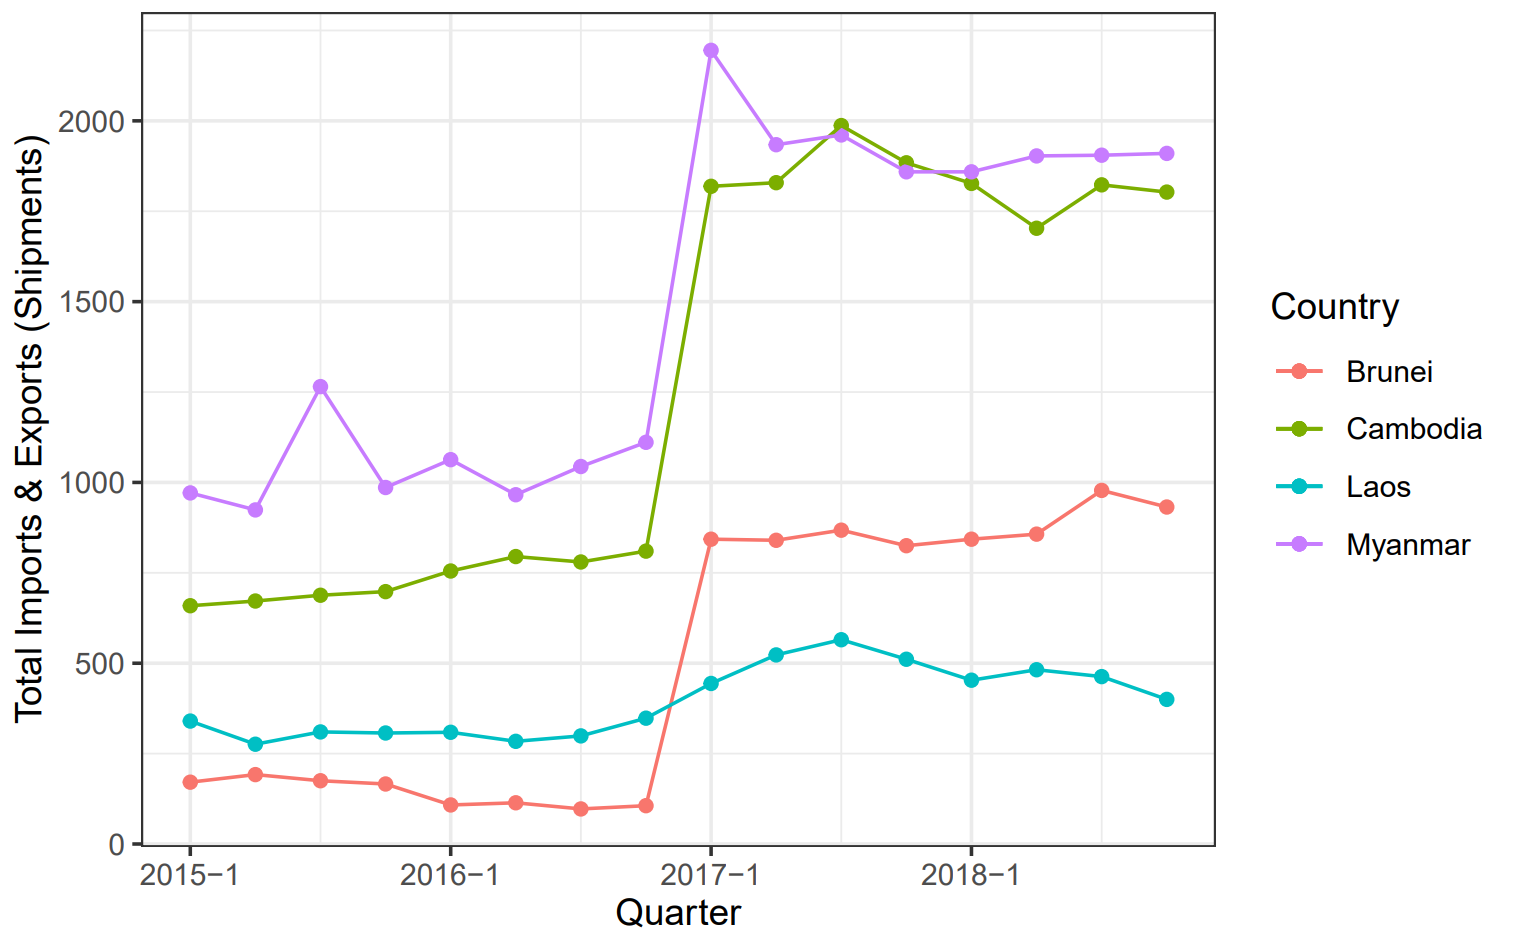
\includegraphics[width=1\textwidth]{images/Line Plots/ASEAN/ASEAN_Small_Quarterly_Shipments.png}
\caption{\label{fig2}Total Shipments for Smaller Activity Countries}
\end{figure}

\noindent Similarly, there is a large increase in the number of shipments from 2016 Q4 to 2017 Q1 for most countries. The only exception to this trend is Laos, where the change in shipment over time seems to be gradual rather than sudden, comparatively.

\subsubsection{Seasonal Trend Analysis}
The line plots below depict the monthly data for the aggregated number of shipments (Imports and Exports) for each country, showing a slight seasonal trend during the months of March to April and October to November. (Should I be using the log-plots or the regular plots? - regular plots show the seasonality better, but obscure the countries with lower activity, vice versa.)

\hspace{1}

\begin{figure}[H]
\centering
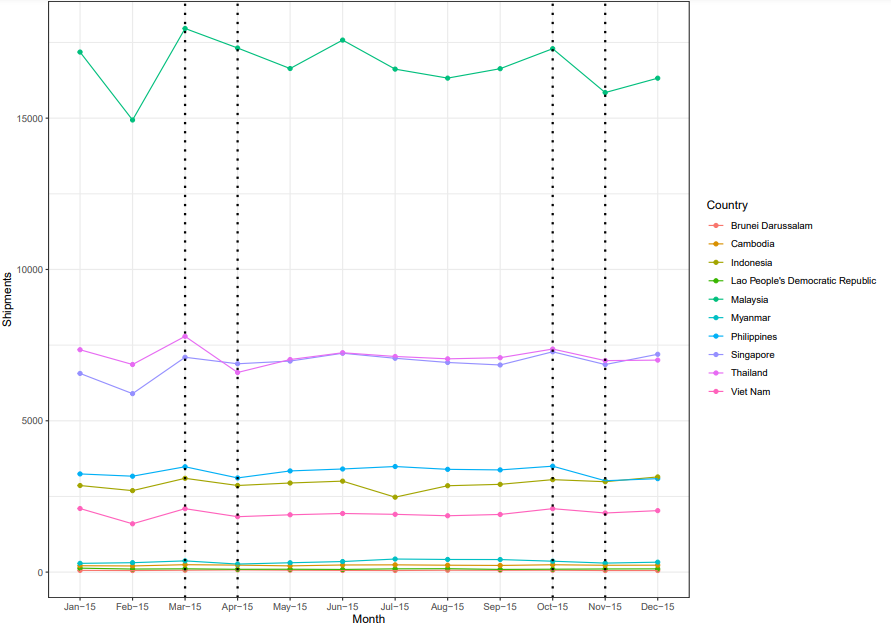
\includegraphics[width=1\textwidth]{images/Line Plots/Seasonal/2015_seasonal.png}
\caption{2015 Monthly Shipments}
\end{figure}

\begin{figure}[H]
\centering
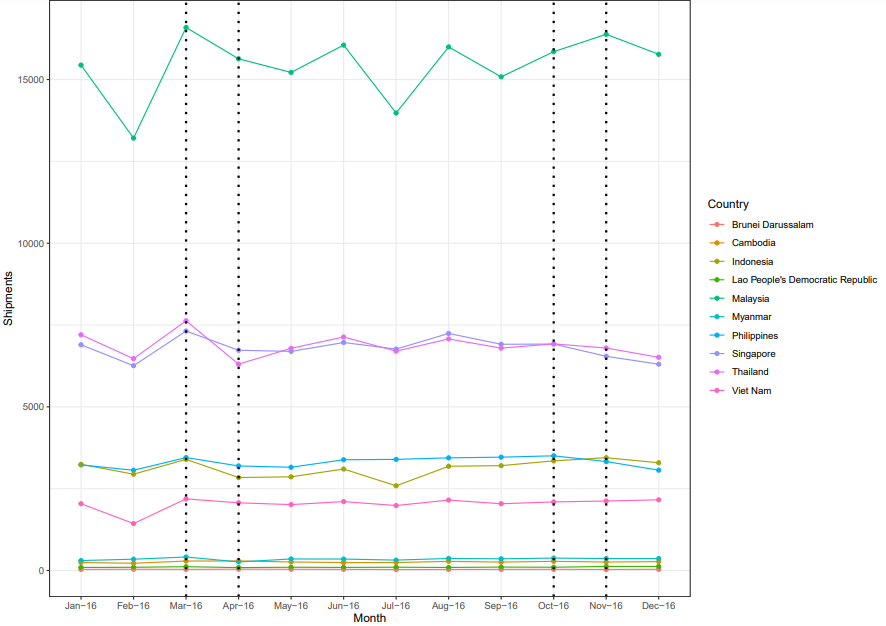
\includegraphics[width=1\textwidth]{images/Line Plots/Seasonal/2016_seasonal.png}
\caption{2016 Monthly Shipments}
\end{figure}

\begin{figure}[H]
\centering
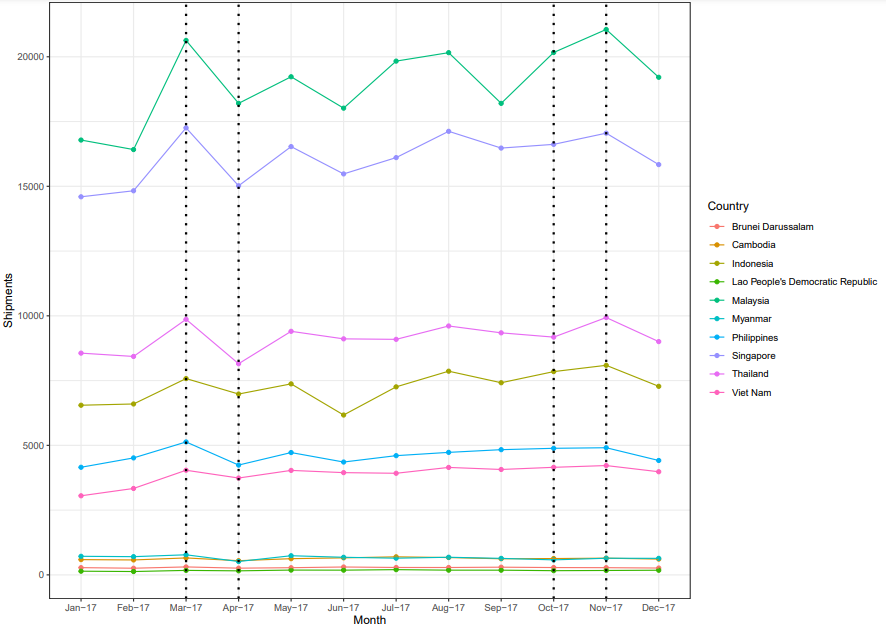
\includegraphics[width=1\textwidth]{images/Line Plots/Seasonal/2017_seasonal.png}
\caption{2017 Monthly Shipments}
\end{figure}

\begin{figure}[H]
\centering
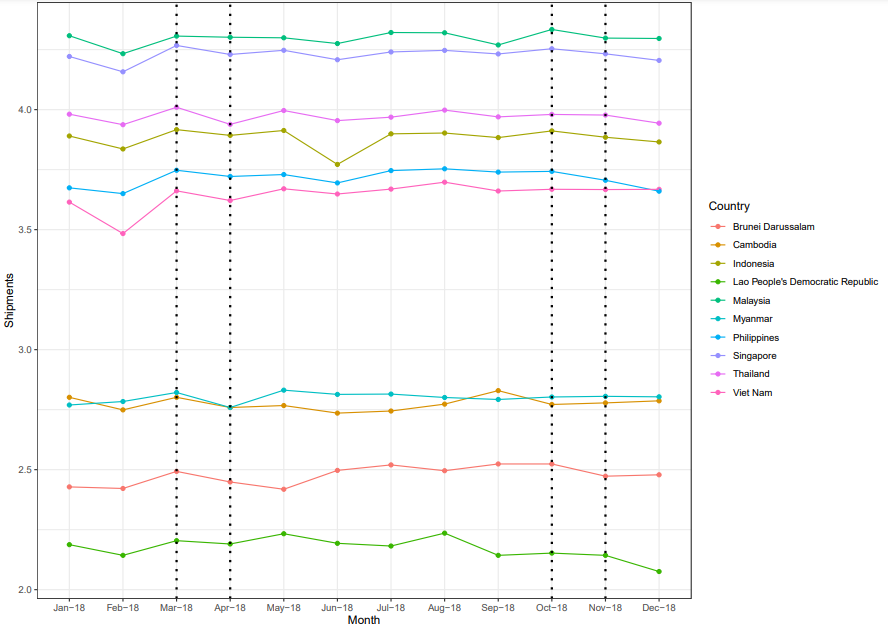
\includegraphics[width=1\textwidth]{images/Line Plots/Seasonal/2018_seasonal.png}
\caption{2018 Monthly Shipments}
\end{figure}

\begin{figure}[H]
\centering
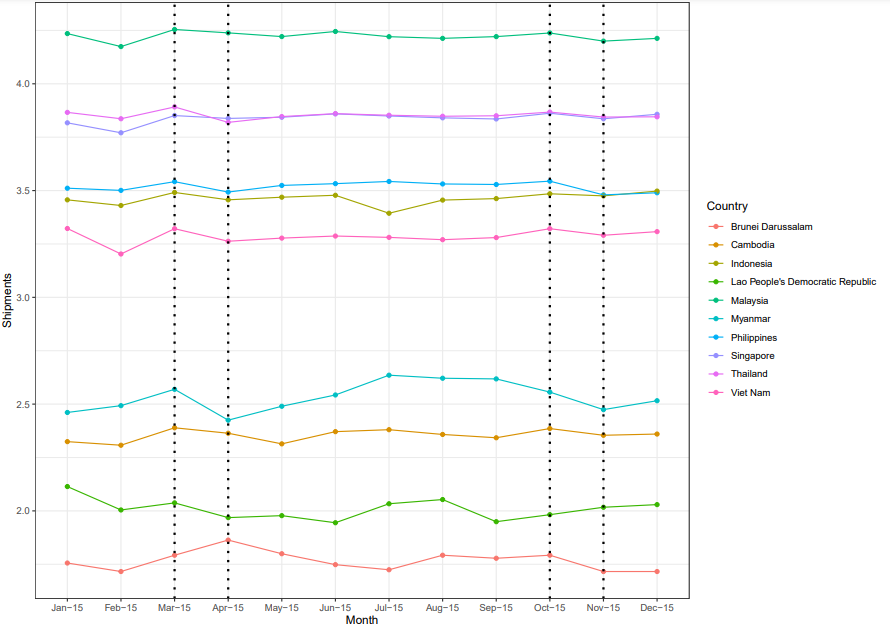
\includegraphics[width=1\textwidth]{images/Line Plots/Seasonal/2015_seasonal_log.png}
\caption{2015 Monthly Shipments (Log)}
\end{figure}

\begin{figure}[H]
\centering
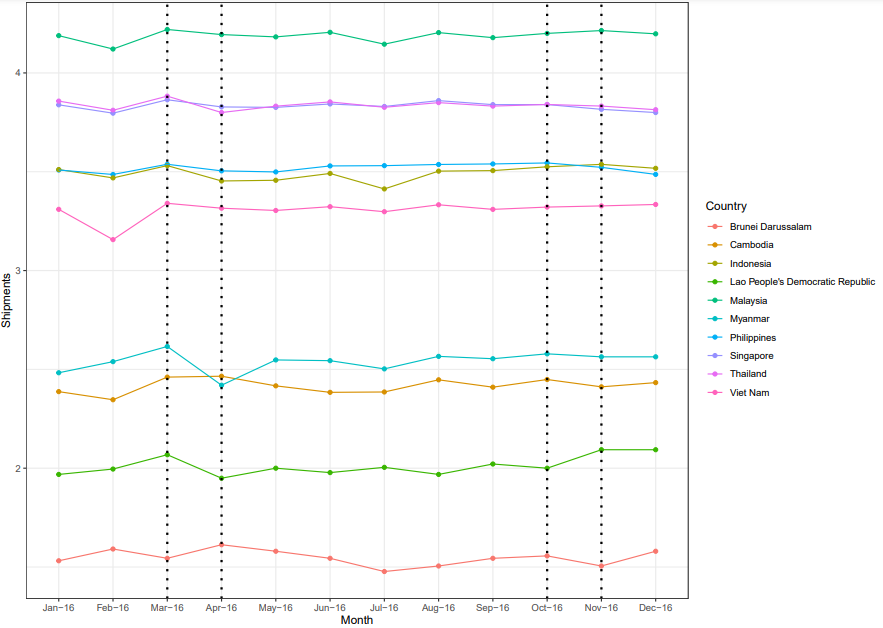
\includegraphics[width=1\textwidth]{images/Line Plots/Seasonal/2016_seasonal_log.png}
\caption{2016 Monthly Shipments (Log)}
\end{figure}

\begin{figure}[H]
\centering
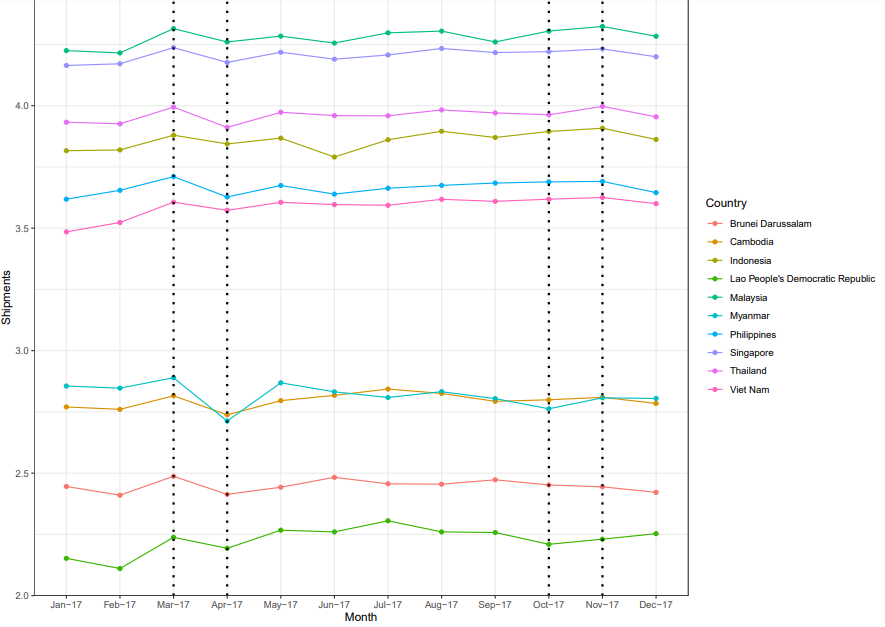
\includegraphics[width=1\textwidth]{images/Line Plots/Seasonal/2017_seasonal_log.png}
\caption{2017 Monthly Shipments (Log)}
\end{figure}

\begin{figure}[H]
\centering
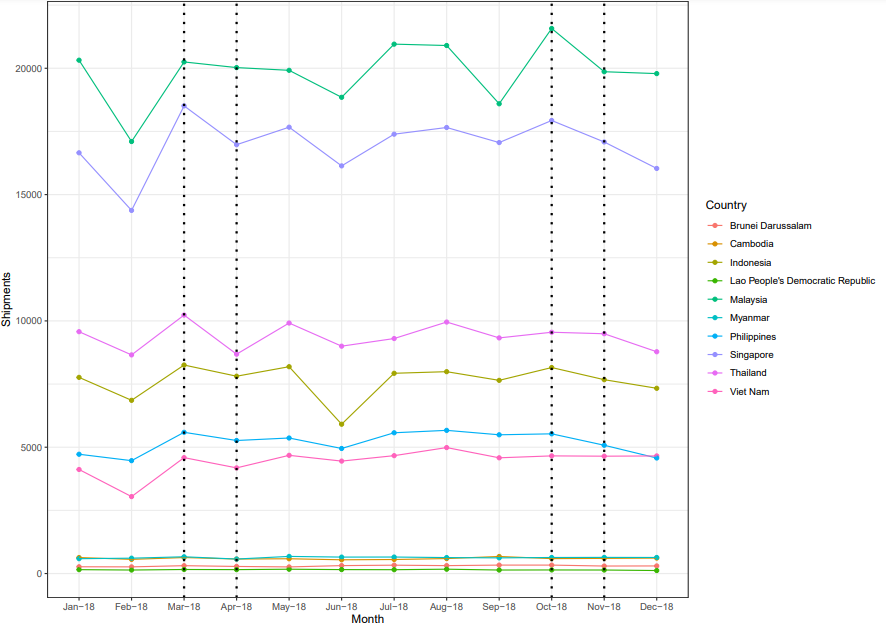
\includegraphics[width=1\textwidth]{images/Line Plots/Seasonal/2018_seasonal_log.png}
\caption{2018 Monthly Shipments (Log)}
\end{figure}

\noindent The figures show a general decrease in the number of shipments from March to April, and similarly from October to November, which is consistent throughout the years. This may be due to ... (to be completed)

\newpage

\section{Identification of Relevant Macroeconomic Data Sources}

A key challenge of the project involves identifying suitable open-source macroeconomic data relevant to the ASEAN region. Analysis will need to be performed to identify the reliability and veracity of such open-source information, particularly for future predictions. The accessibility and availability of such data will also need to be established to assess the ongoing capability of using such information in future air cargo demand forecasting. \\

\noindent In the course of the project, we developed hypotheses about what macroeconomic factors could be of influence on air cargo demand, and how different sets of macroeconomic factors might be related to each other. This will be detailed in the following sections. \\

\noindent There exists a multitude of macroeconomic datasets online, many of which are paywalled or non-accessible to public use without proper licensing. Thus, our identification of relevant macroeconomic data is limited to open-source data and existing subscriptions provided by institutions. The main sources of datasets which we had access to are the following:

\begin{itemize}
    \item \href{https://data.worldbank.org/}{World Bank Group} 
    \item \href{https://data.imf.org}{International Monetary Fund (IMF)}
    \item \href{https://statista.com}{Statista (Existing Subscription)}
\end{itemize} 

\subsection{Data Cleaning}
Since we are working with open-source macroeconomic datasets, there is a significant inconsistency in the formatting of each country's datasets. Thus, we had to employ further data cleaning techniques to re-order the data for our use. As we were sourcing for quarterly data, the indicators for each country had to be collated into an Excel sheet manually, and reordered based on the given time range.

\subsection{Macroeconomic Indicators}
Our main source of macroeconomic data used is obtained from each country's respective department of statistics, whereby an online open-sourced repository of the country's data is stored. This usually includes the country's National Accounts, as well as data obtained from nation-wide surveys on various indicators such as mean household income. \\

\noindent Some of the macroeconomic indicators which we sourced for initially included the \textit{Balance of Payments (BoP)}, \textit{Gross Domestic Product (GDP)}, \textit{Consumer Price Index (CPI)}, and others such as the \textit{Percentage of Population with Internet Access}. \\

\noindent Each country's department of statistics' portal can be found in the links below:

\begin{multicols}{2}
    \begin{itemize} 
        \item \href{https://www.singstat.gov.sg/}{Singapore}
        \item \href{https://www.data.gov.my/}{Malaysia}
        \item \href{https://www.nesdc.go.th/nesdb_en/main.php?filename=index}{Thailand}
        \item \href{https://psa.gov.ph/}{Philippines}
        \item \href{https://www.bps.go.id/}{Indonesia}
    \end{itemize}
    
    \columnbreak
    
    \begin{itemize}
        \item \href{https://www.gso.gov.vn/en/homepage/}{Vietnam}
        \item \href{https://deps.mofe.gov.bn/Theme/Home.aspx}{Brunei}
        \item \href{https://www.lsb.gov.la/en/home/}{Laos}
        \item \href{https://www.mmsis.gov.mm/}{Myanmar}
        \item \href{https://www.nis.gov.kh/index.php/km/}{Cambodia}
    \end{itemize}

\end{multicols} \\

\noindent The macroeconomic data sourced was aggregated in quarters (if given), to align with the CargoIS data which was cleaned as aforementioned. 


\subsubsection{Gross Domestic Product}
GDP, as defined by the IMF, is the monetary value of final goods and services purchased by the user, and produced in a country in a given period of time. The line plots of each country's GDP aggregated in quarters per year is given below, in contrast with their aggregated shipments. Only GDP values for the countries below have been found aggregated quarterly from the respective National Statistics Departments, while the rest only include data aggregated annually.

\newpage

\begin{figure}[h]%
    \centering
    \subfloat[\centering Singapore's Aggregated Shipments]{{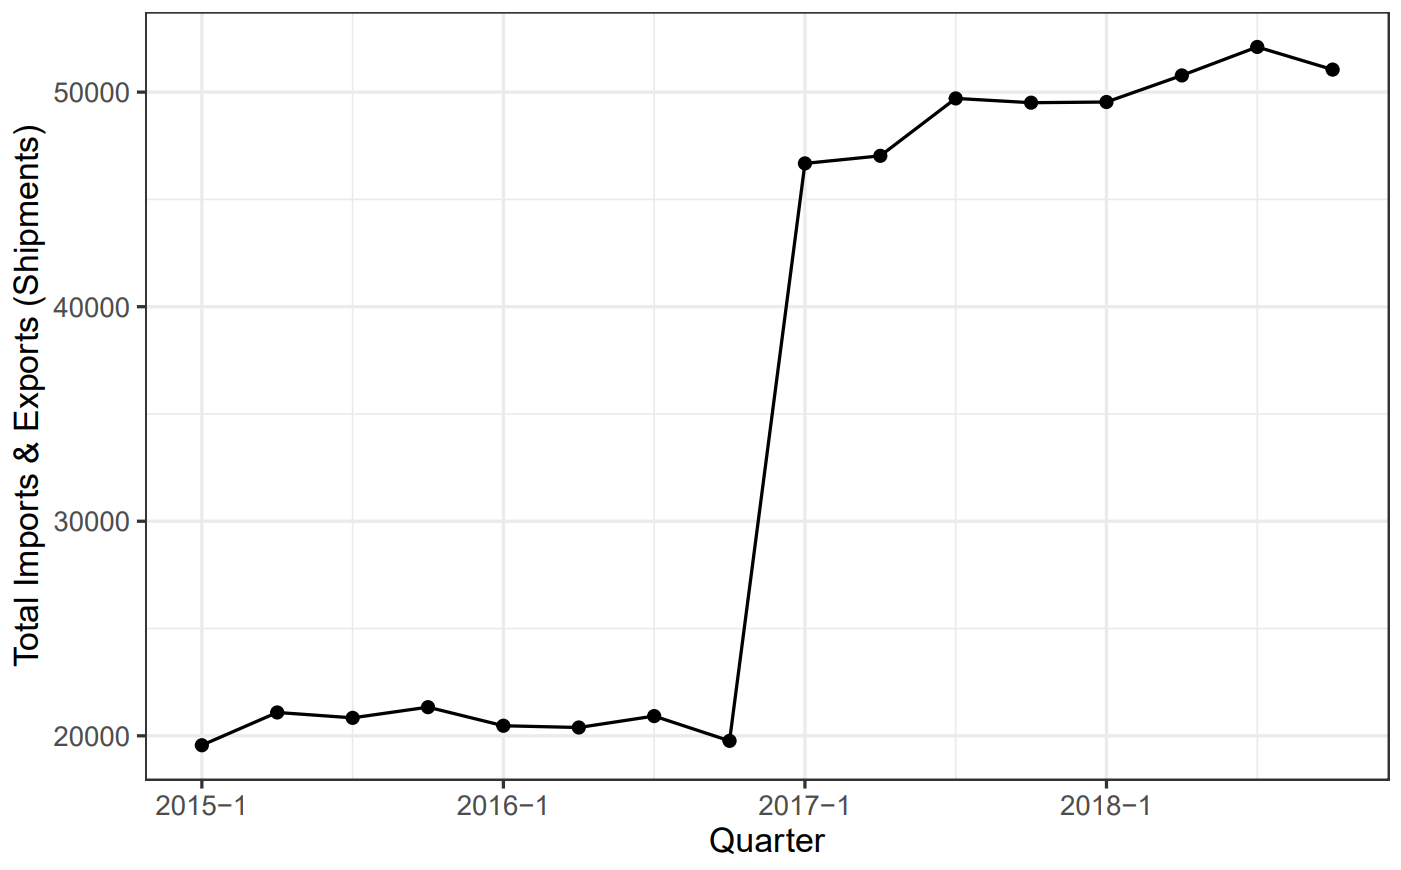
\includegraphics[width=0.45\textwidth]{images/Line Plots/Singapore/SG_Shipments_Quarter.png} }}%
    \qquad
    \subfloat[\centering Singapore's GDP]{{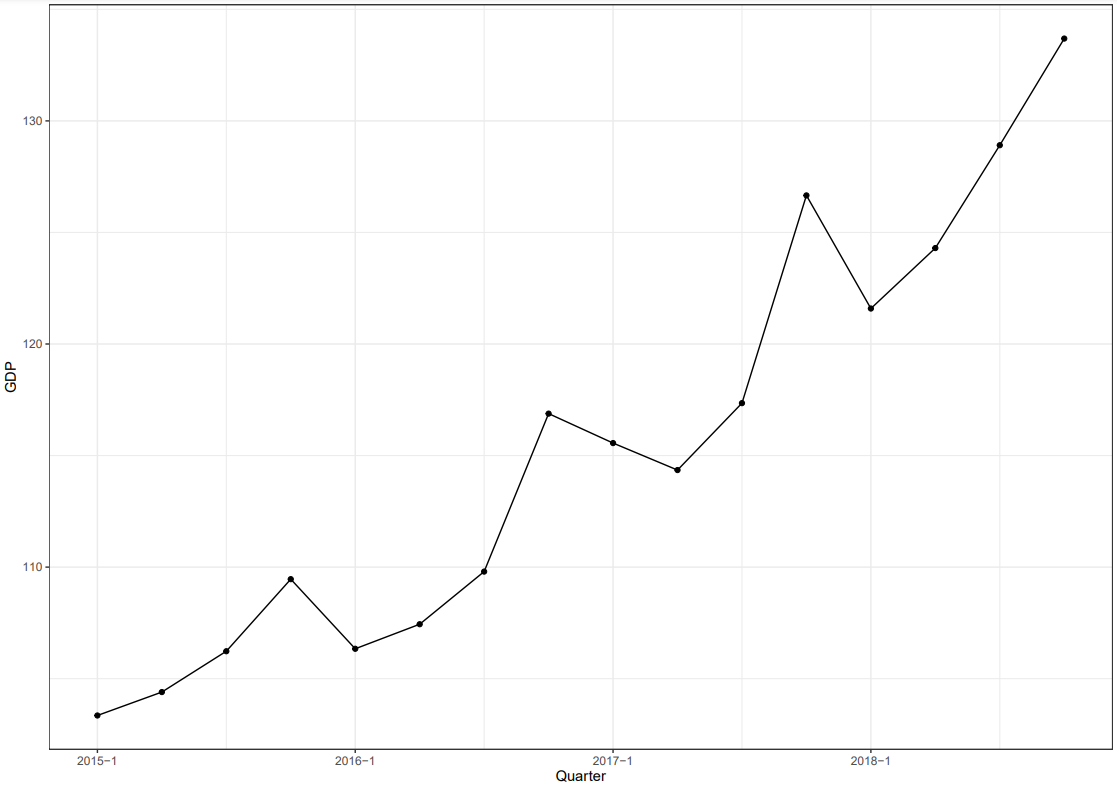
\includegraphics[width=0.45\textwidth]{images/Line Plots/Singapore/SG_GDP_Quarter.png}}}%
    \caption{Singapore}%
    \label{fig: sggdp}%
\end{figure}

% \noindent Aggregate value of the goods and services produced in the economic territory of Singapore. The GDP estimates are compiled based on the output (or production), expenditure and income approaches.

\begin{figure}[H]
    \centering
    \subfloat[\centering Philippines' Aggregated Shipments]{{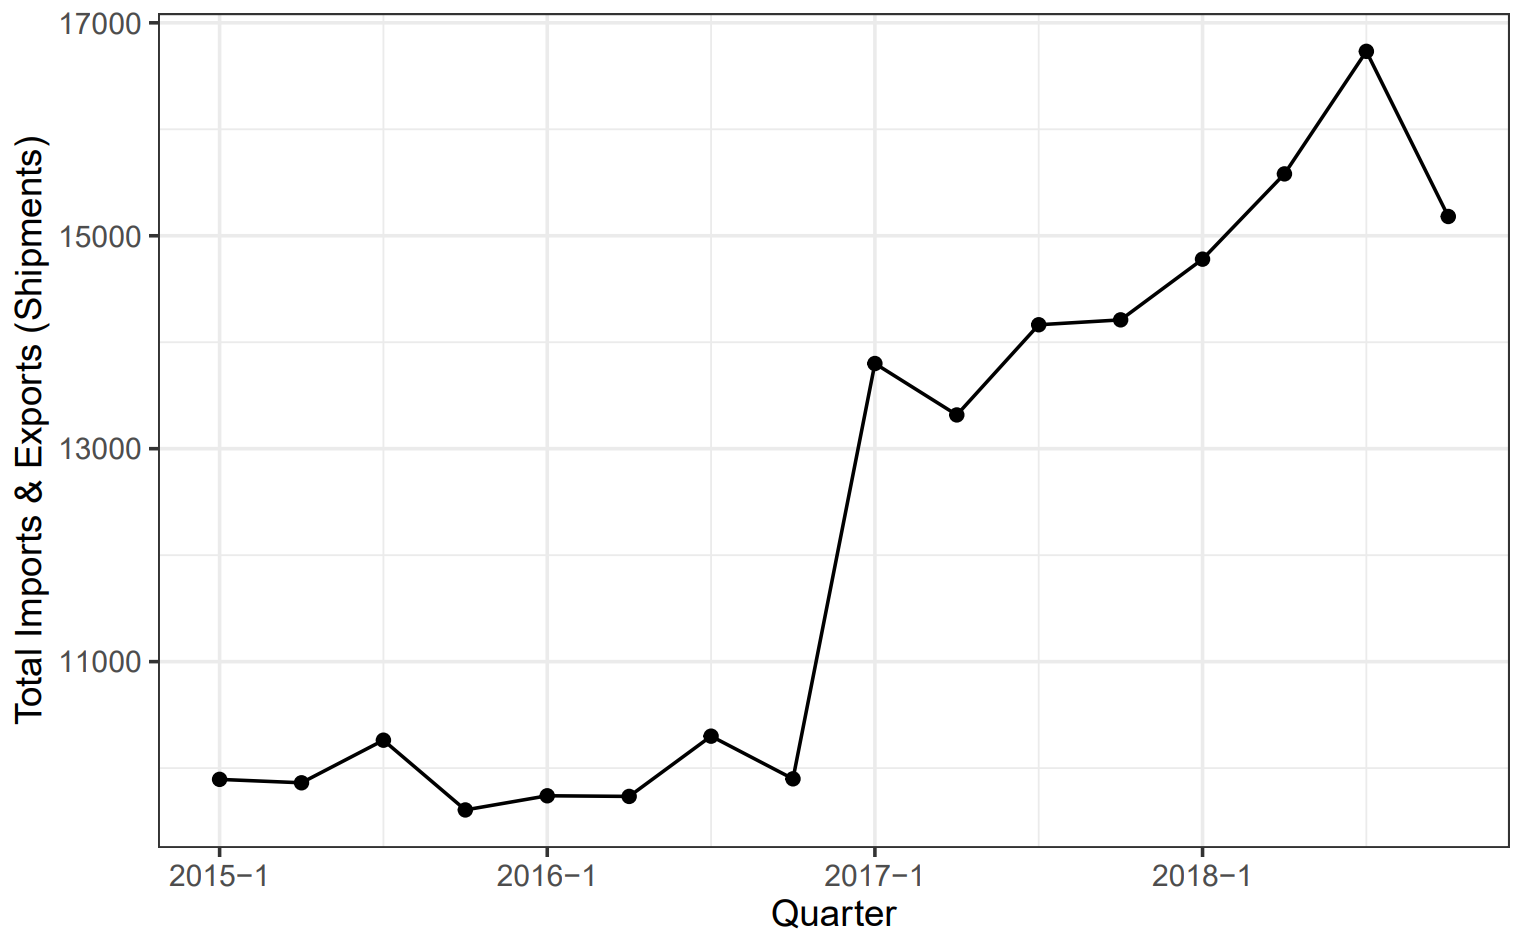
\includegraphics[width=0.45\textwidth]{images/Line Plots/Philippines/PH_Quarterly_Shipments.png} }}
    \qquad
    \subfloat[\centering Philippines' GDP]{{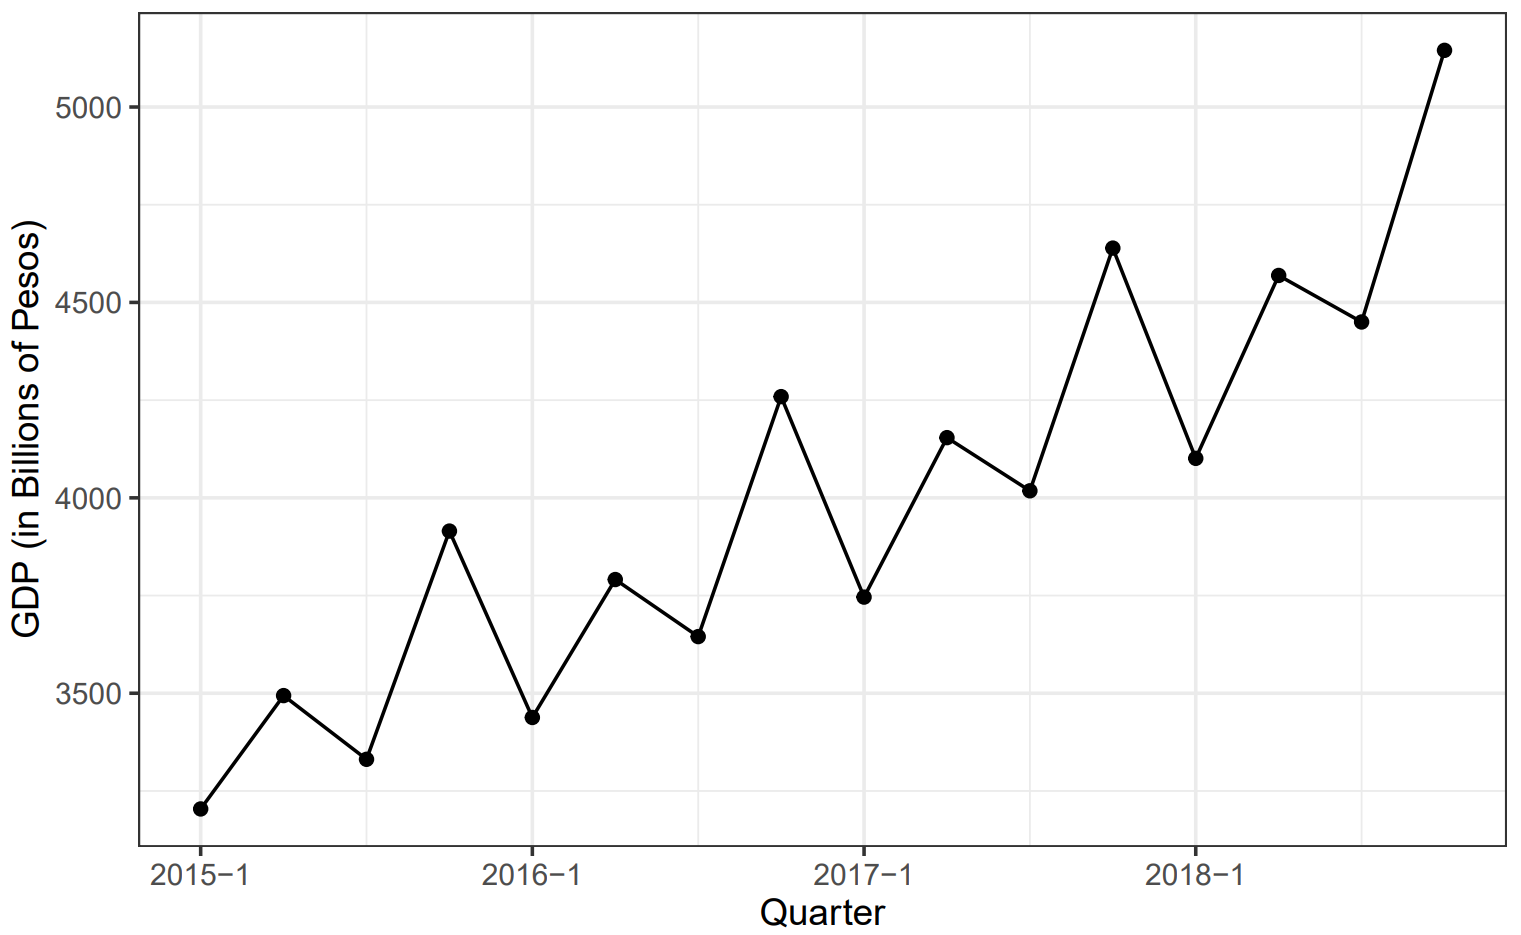
\includegraphics[width=0.45\textwidth]{images/Line Plots/Philippines/PH_Quarterly_GDP.png}}}
    \caption{Philippines}
    \label{fig: phgdp}
\end{figure}

\begin{figure}[H]
    \centering
    \subfloat[\centering Thailand's Aggregated Shipments]{{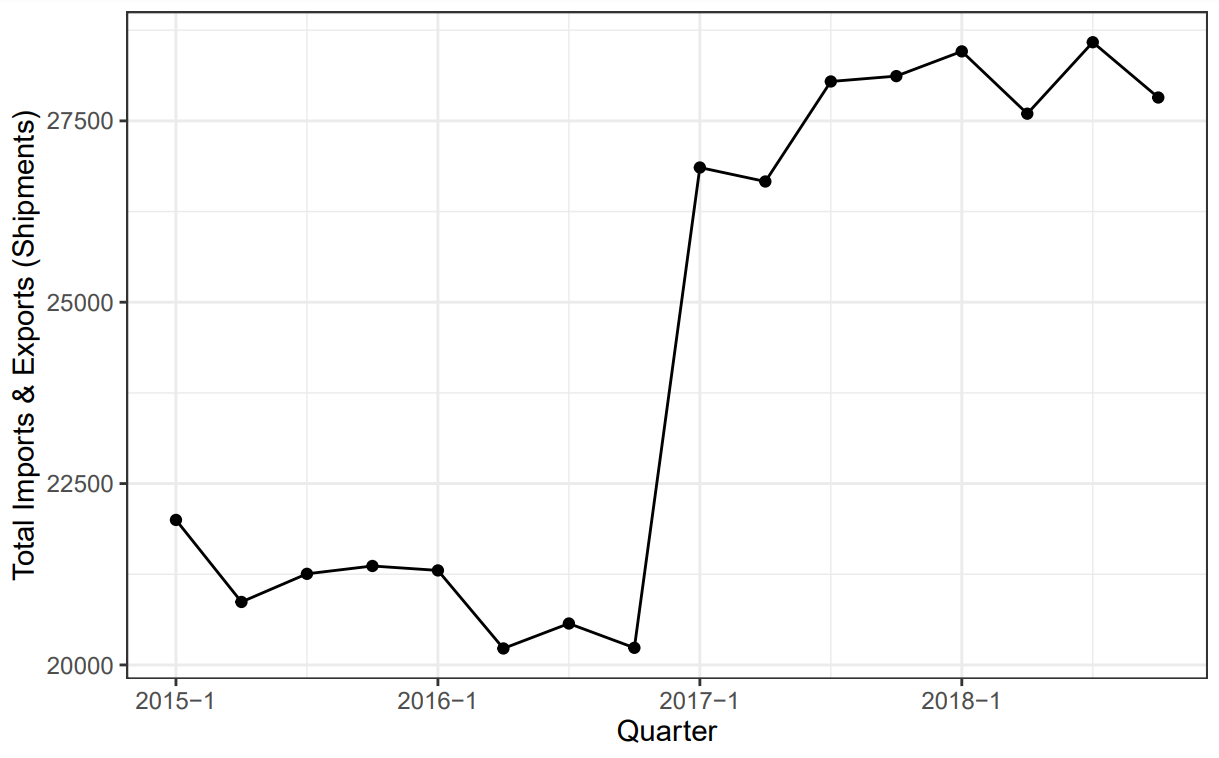
\includegraphics[width=0.45\textwidth]{images/Line Plots/Thailand/Thai_Quarterly_Shipments.png} }}
    \qquad
    \subfloat[\centering Thailand's GDP]{{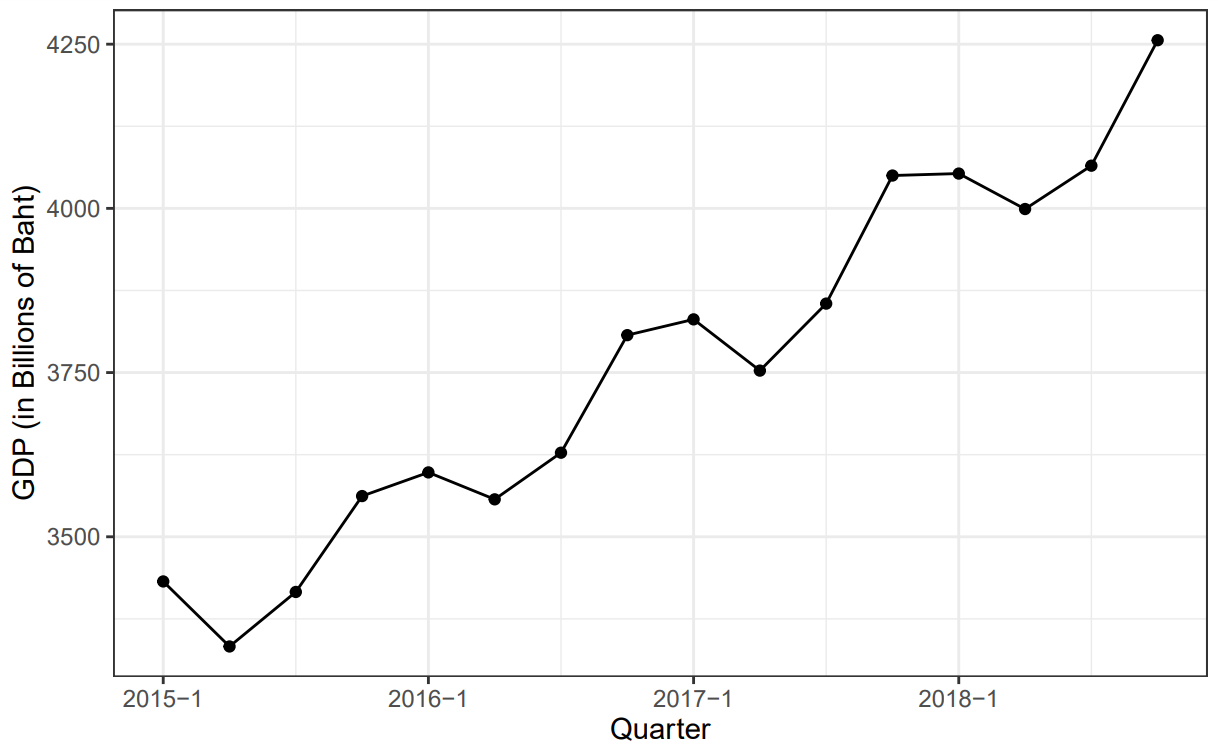
\includegraphics[width=0.45\textwidth]{images/Line Plots/Thailand/Thai_Quarterly_GDP.png}}}
    \caption{Thailand}
    \label{fig: thgdp}
\end{figure}

\begin{figure}[H]
    \centering
    \subfloat[\centering Malaysia's Aggregated Shipments]{{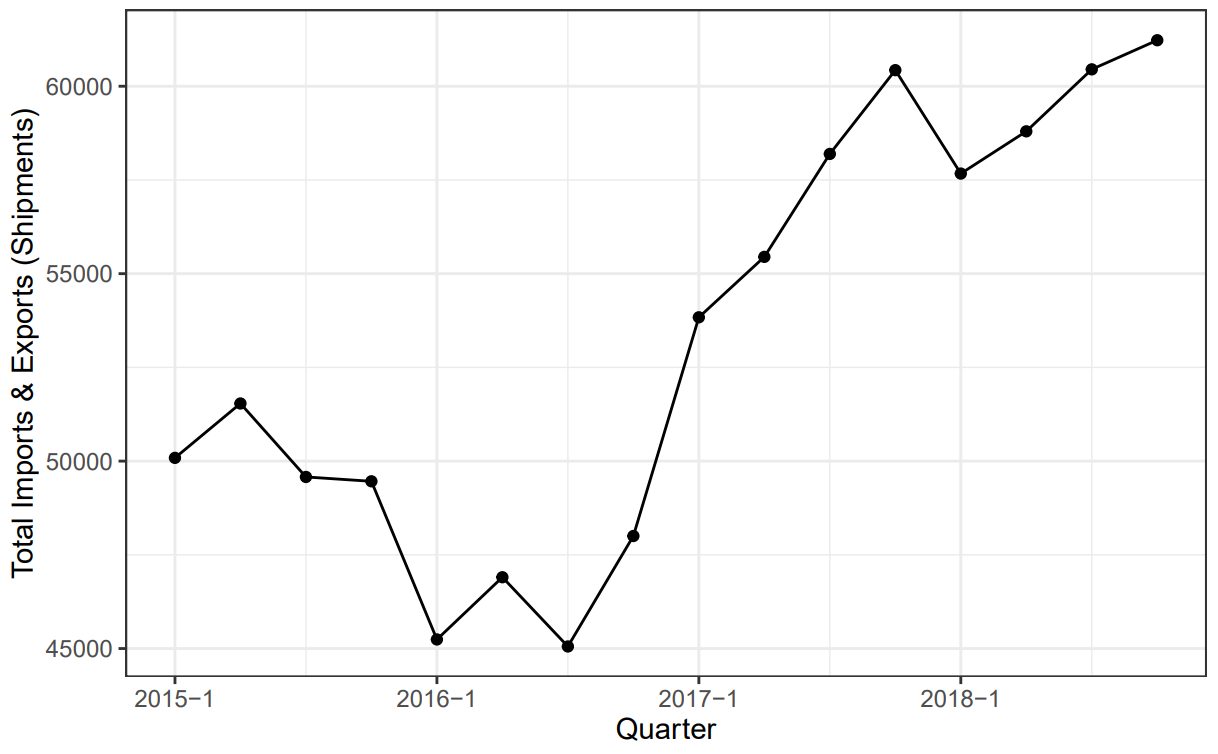
\includegraphics[width=0.45\textwidth]{images/Line Plots/Malaysia/MY_Quarterly_Shipments.png} }}
    \qquad
    \subfloat[\centering Malaysia's GDP]{{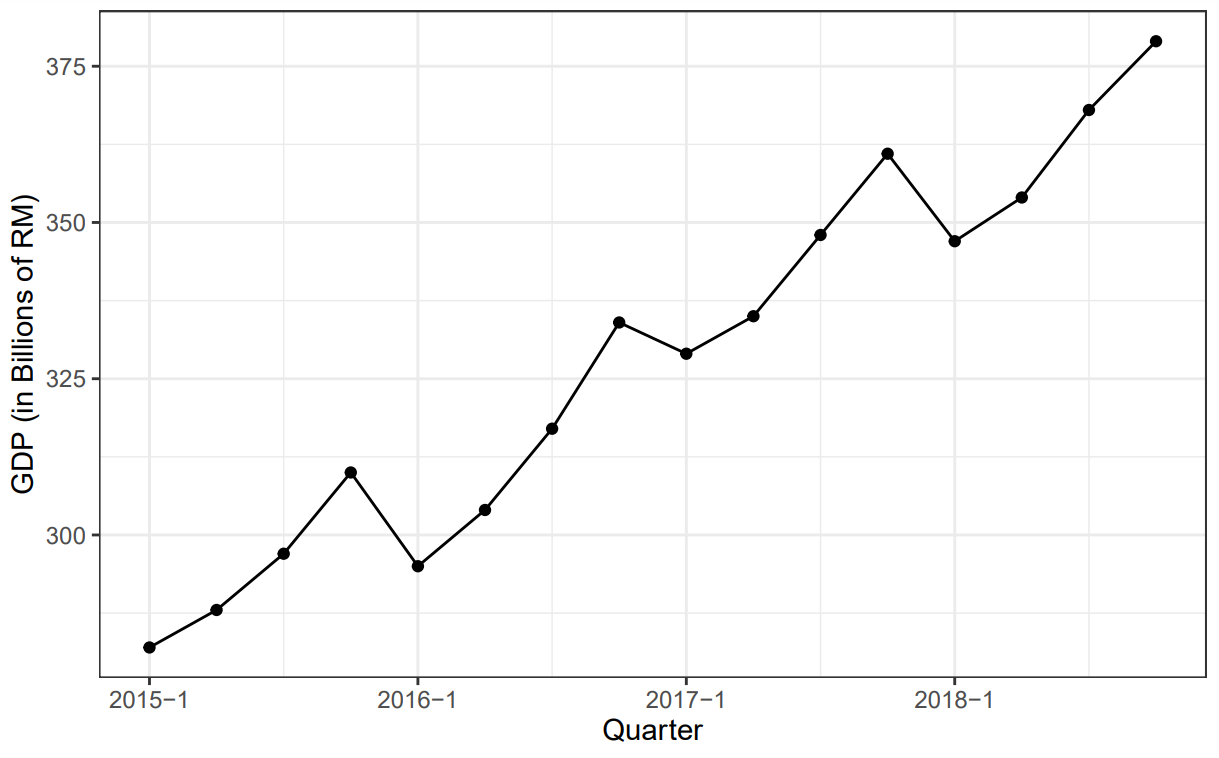
\includegraphics[width=0.45\textwidth]{images/Line Plots/Malaysia/MY_GDP_Quarterly.png}}}
    \caption{Malaysia}
    \label{fig: mygdp}
\end{figure}

\begin{figure}[H]
    \centering
    \subfloat[\centering Indonesia's Aggregated Shipments]{{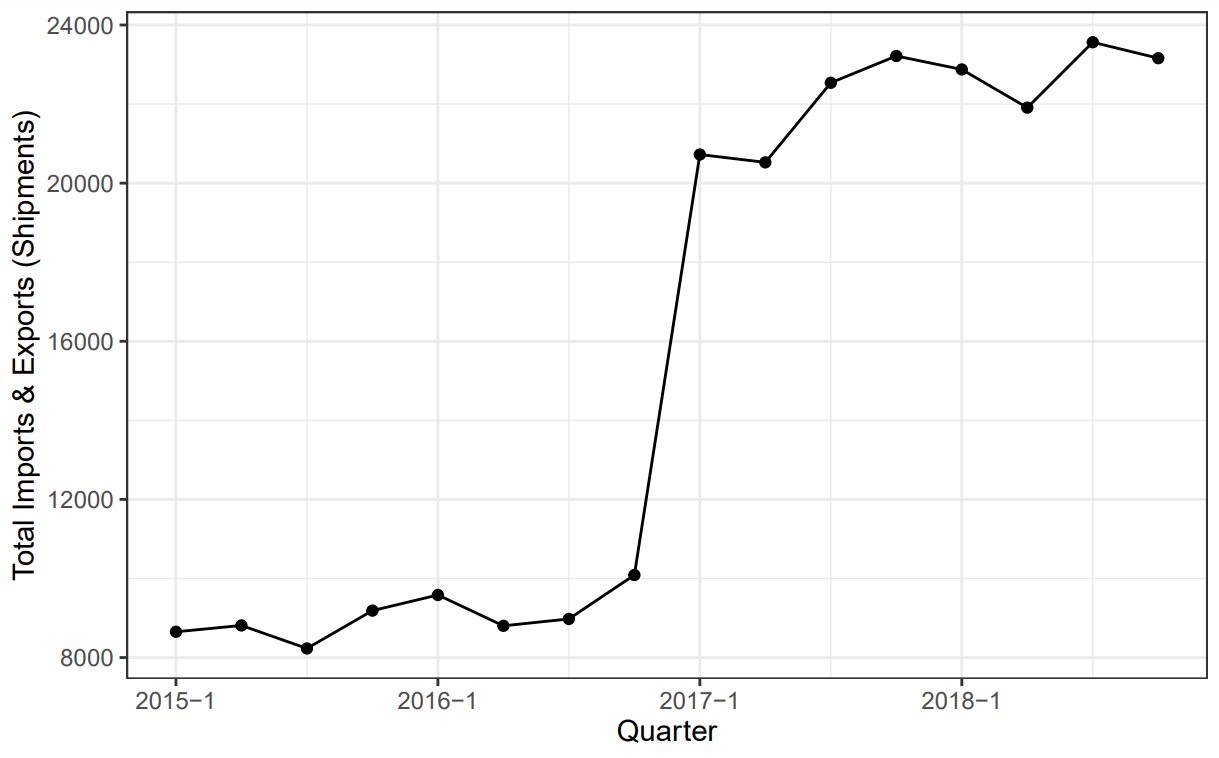
\includegraphics[width=0.45\textwidth]{images/Line Plots/Indonesia/Indonesia_Shipments.png}}}
    \qquad
    \subfloat[\centering Indonesia's GDP (Statista)]{{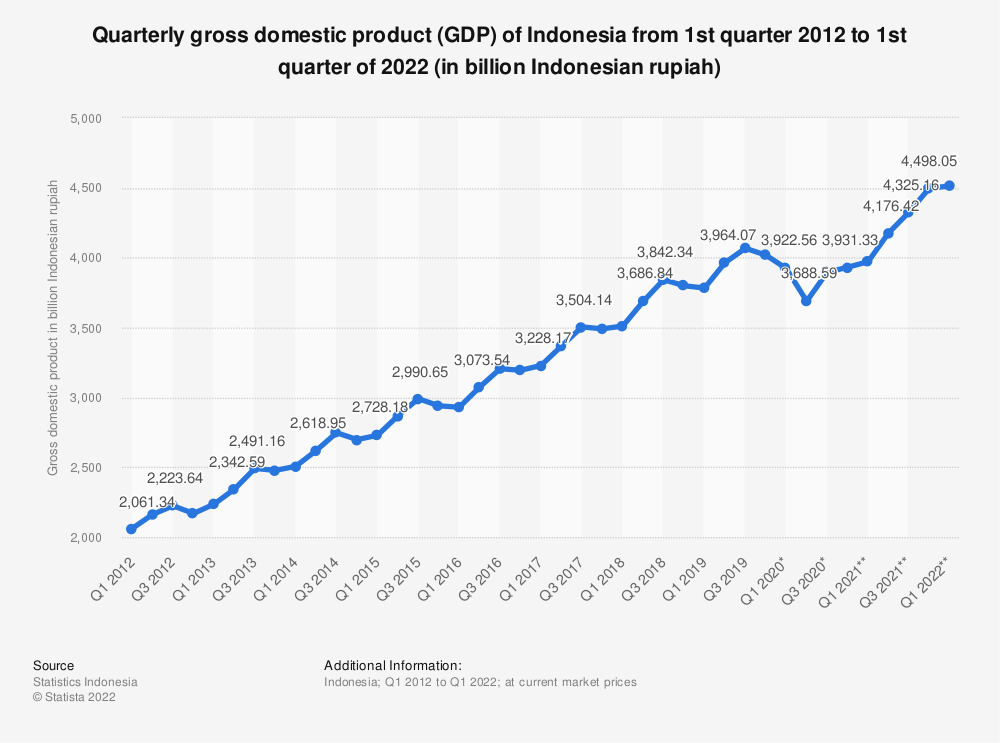
\includegraphics[width=0.45\textwidth]{images/Line Plots/Indonesia/Indonesia_GDP.png}}}
    \caption{Indonesia}
    \label{fig: mygdp}
\end{figure}

\begin{figure}[H]
    \centering
    \subfloat[\centering Brunei's Aggregated Shipments]{{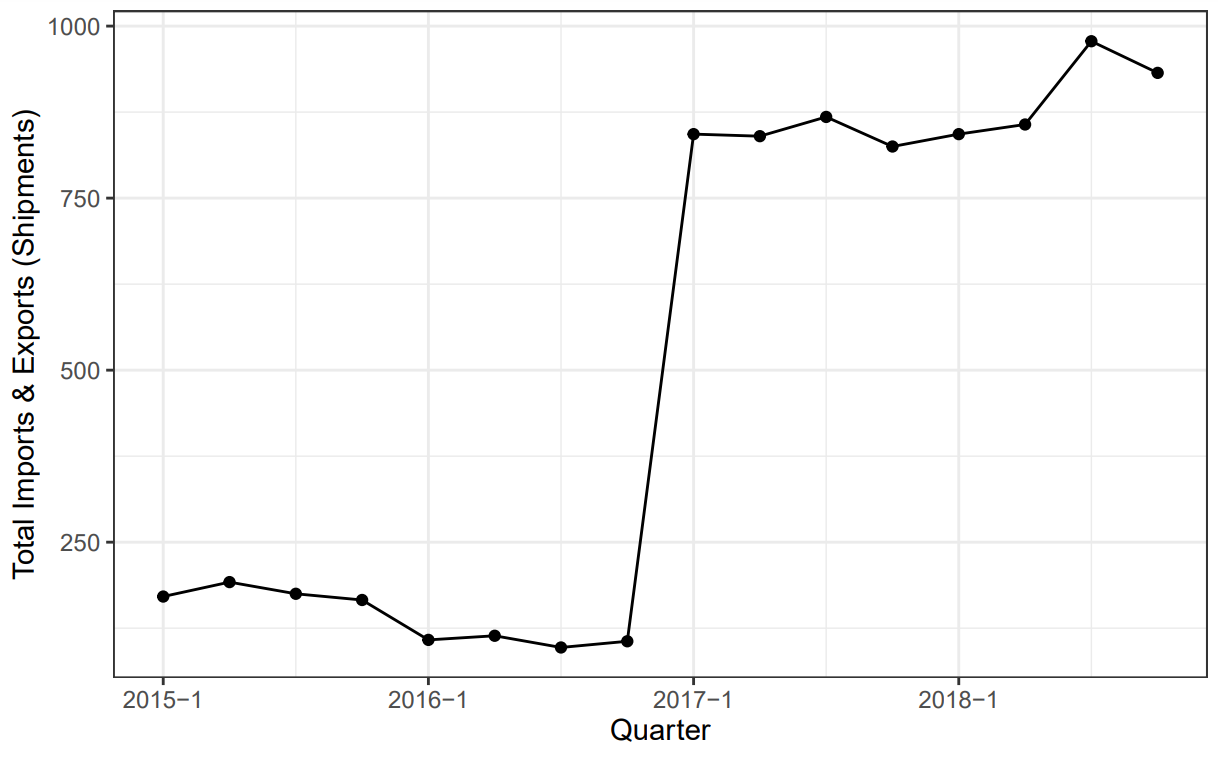
\includegraphics[width=0.45\textwidth]{images/Line Plots/Brunei/Brunei_Shipments_Quarterly.png}}}
    \qquad
    \subfloat[\centering Brunei's GDP]{{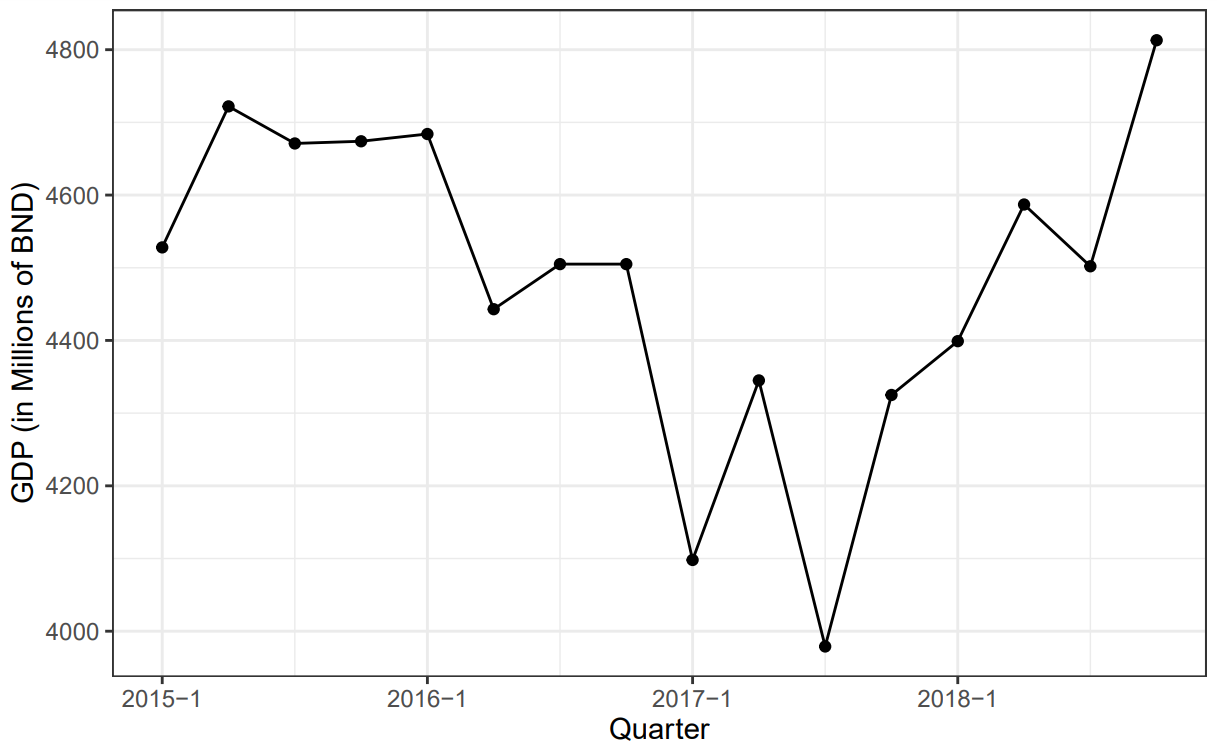
\includegraphics[width=0.45\textwidth]{images/Line Plots/Brunei/Brunei_GDP_Quarterly.png}}}
    \caption{Brunei}
    \label{fig: mygdp}
\end{figure}

\noindent For most countries, there is visually a general increase in the GDP over time, whilst the shipments for each country pre-2017 stayed relatively consistent or decreased slightly. Post-2017 however, there seems to be a slight increase over the quarters. Brunei is the only exception to this trend, where its GDP decreased from 2016 to 2017. We suspect this to be due to the oil price collapse in 2016, which largely affected the Brunei economy. 

\newpage


% \subsubsection{Government Debt}
% We have also obtained data describing the local government debt of all countries by quarter (ignore first)

% \begin{figure}[H]
% \centering
% 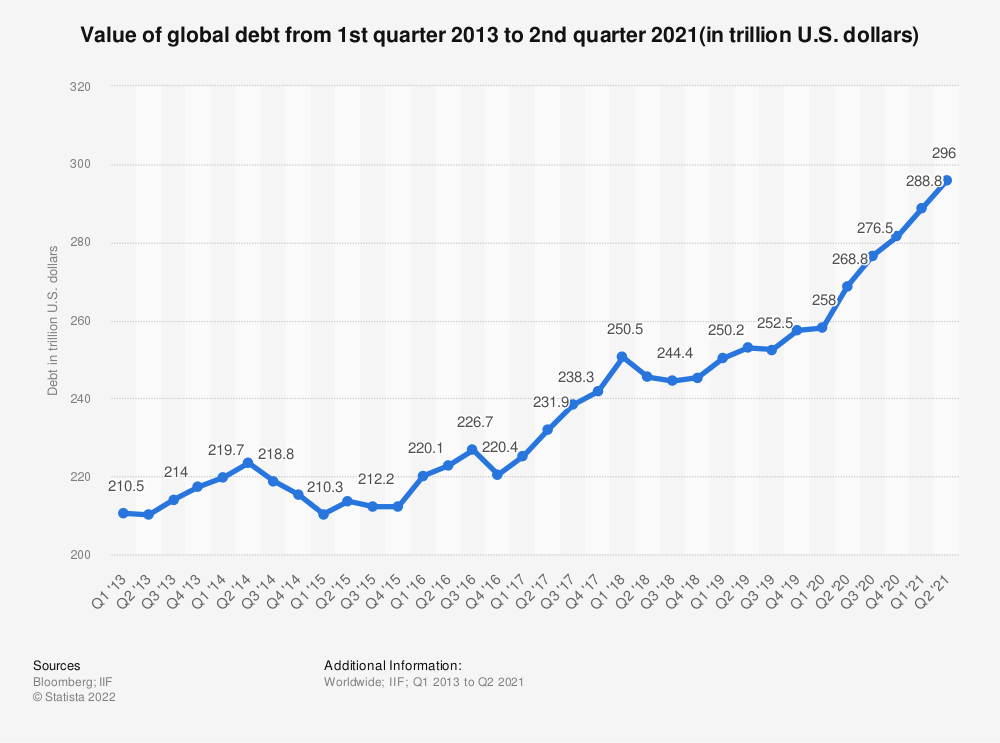
\includegraphics[width=0.8\textwidth]{images/Line Plots/Global Debt/Global_Debt.png}
% \caption{\label{fig2}Global Debt Values}
% \end{figure}

\subsection{Analysis of Data Credibility}
Include cross-referencing with World Bank database if we have the time, though unlikely.

\subsection{Correlation of Cargo Data with Macroeconomic Data}

As our dataset is too small to be conducting any meaningful regression analysis, we have decided to proceed with correlation analysis with the given 16 data points. 

\subsubsection{Pearson's Correlation Coefficient}
The Pearson's Correlation Coefficient is a statistical measure of linear correlation between two sets of data. Mathematically, it is the covariance of the two variables divided by the product of their standard deviations. When applied to a sample with bivariate data of $n$ pairs, the formula is given by \\

\begin{equation}
    r = \frac{ \sum_{i=1}^{n}(x_i-\bar{x})(y_i-\bar{y}) }{%
        \sqrt{\sum_{i=1}^{n}(x_i-\bar{x})^2}\sqrt{\sum_{i=1}^{n}(y_i-\bar{y})^2}}
\end{equation} \\

\noindent The correlation coefficient ranges from $-1$ to $1$. An absolute value of exactly $1$ implies that a linear equation describes the relationship between $X$ and $Y$ perfectly, while the sign denotes positive or anti-correlation. \\

\noindent Correlation plots (Pair Plots in $R$) are shown below, between the macroeconomic indicator and the number of shipments of each country, along with the Pearson's correlation value in the upper right matrix. Plots along the diagonal represent the density distribution plot of Shipment or GDP correspondingly. These plots are obtained via kernel density estimates to show the probability density function of each variable, and are essentially smoothed-out histogram plots.

\begin{figure}[H]
    \centering
    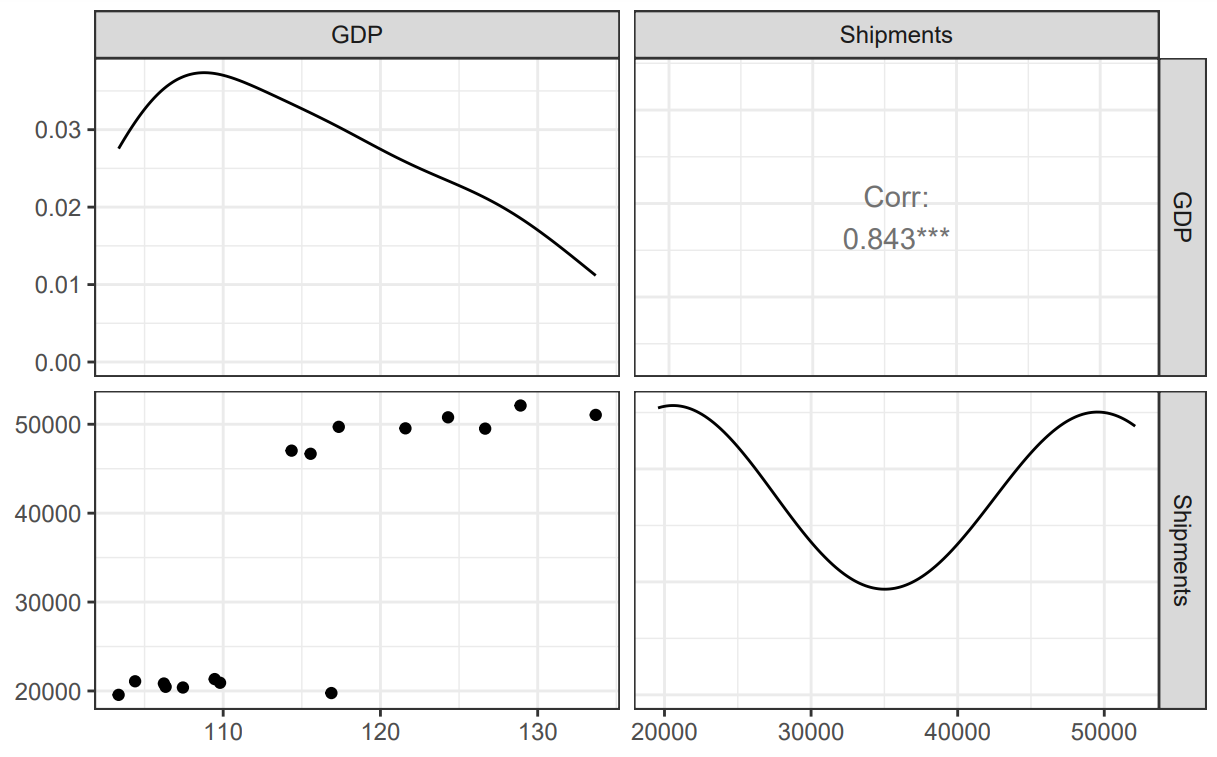
\includegraphics[width=1\textwidth]{images/Line Plots/Singapore/Singapore_Corrplot.png}
    \caption{Singapore GDP Correlation Plot}
    \label{fig:my_label}
\end{figure}

\begin{figure}[H]
    \centering
    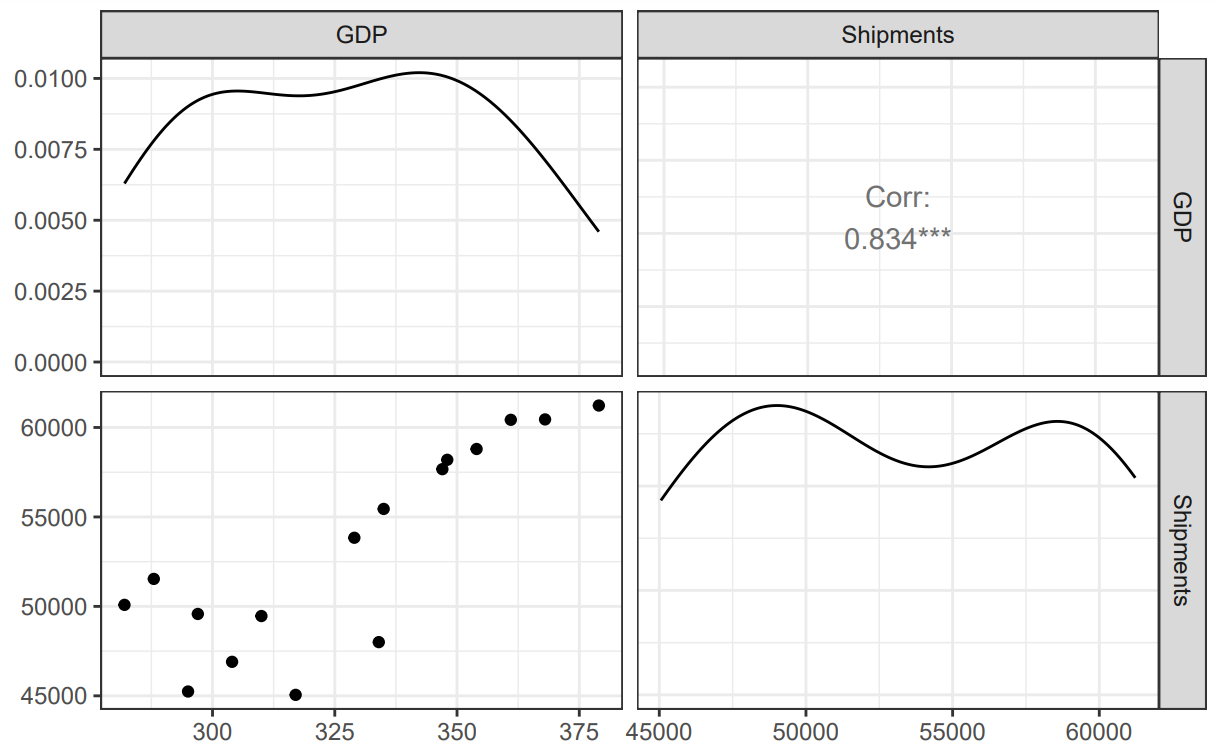
\includegraphics[width=1\textwidth]{images/Line Plots/Malaysia/Malaysia_Corrplot.png}
    \caption{Malaysia GDP Correlation Plot}
    \label{fig:my_label}
\end{figure}

\begin{figure}[H]
    \centering
    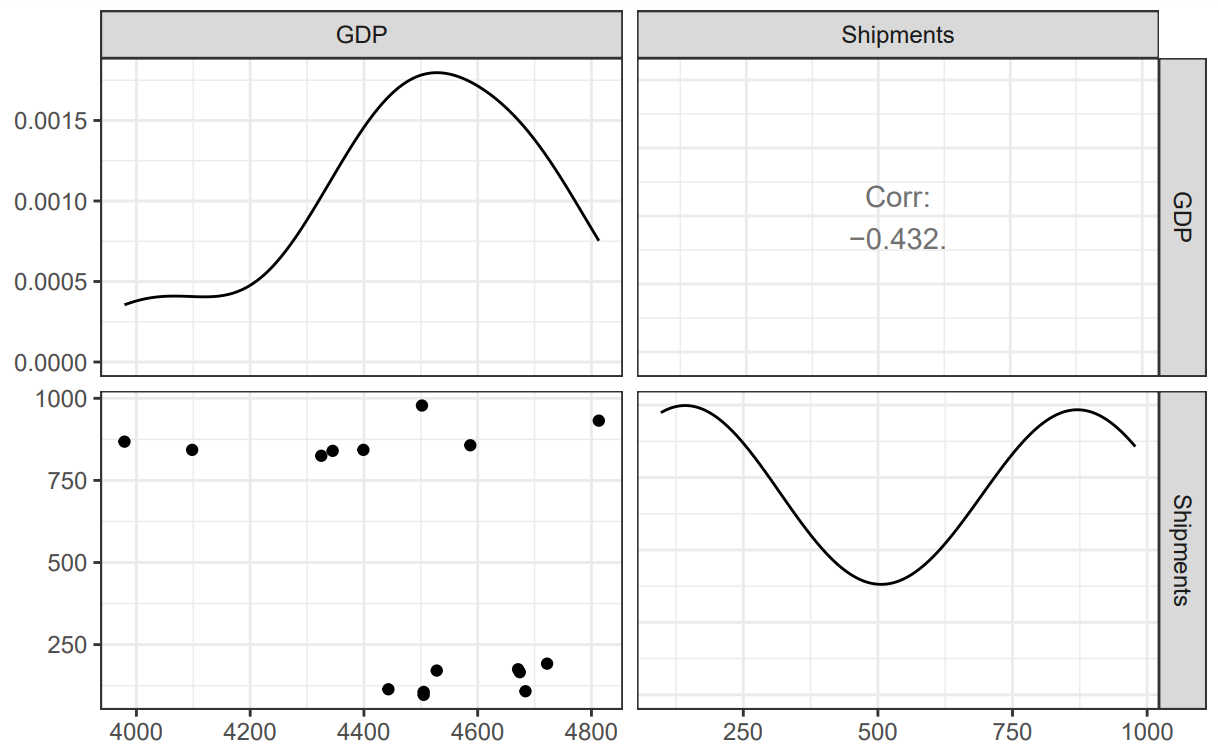
\includegraphics[width=1\textwidth]{images/Line Plots/Brunei/Brunei_Corrplot.png}
    \caption{Brunei GDP Correlation Plot}
    \label{fig:my_label}
\end{figure}

\begin{figure}[H]
    \centering
    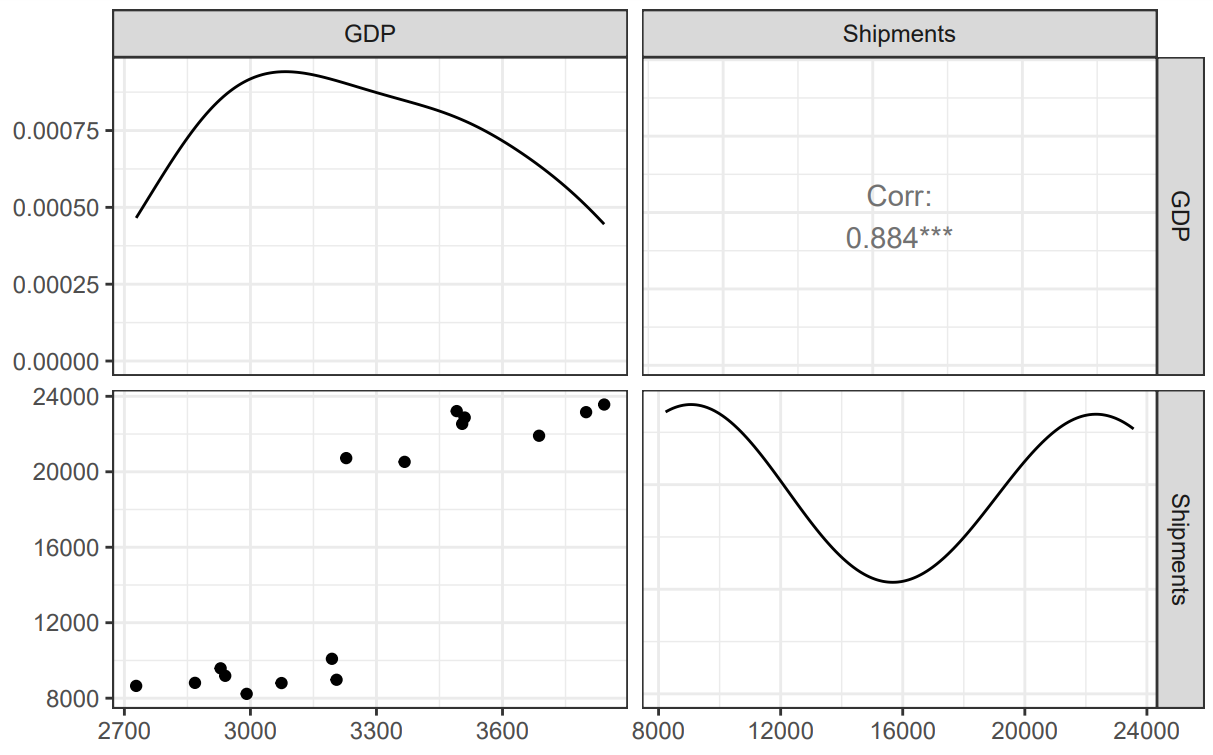
\includegraphics[width=1\textwidth]{images/Line Plots/Indonesia/Indonesia_Corrplot.png}
    \caption{Indonesia GDP Correlation Plot}
    \label{fig:my_label}
\end{figure}

\begin{figure}[H]
    \centering
    \includegraphics[width=1\textwidth]{images/Line Plots/Philippines/Philippines_Corrplot.png}
    \caption{Philippines GDP Correlation Plot}
    \label{fig:my_label}
\end{figure}

\begin{figure}[H]
    \centering
    \includegraphics[width=1\textwidth]{images/Line Plots/Thailand/Thailand_Corrplot.png}
    \caption{Thailand GDP Correlation Plot}
    \label{fig:my_label}
\end{figure}

\noindent Notable trends include the similar shape of each density distribution of the shipments for all countries, which indicates that most countries tend to either engage in trade with very large or small number of shipments, but little in-between. \\

\noindent Another interesting observation is the \textit{relatively} high correlation values for each country (excluding Brunei), suggesting possibly a correlation between the GDP values of a country and its corresponding shipments. 

\subsubsection{Hypothesis Testing}
For us to determine whether the correlation values are statistically significant, we shall employ hypothesis testing on the correlation coefficient obtained. To measure the significance of our empirical analyses, we will use the \textbf{\textit{p-value}}, which is defined as the probability of obtaining results ‘as extreme’ or ‘more extreme’, under the assumption that the null hypothesis is true. The lower the p-value, the higher the significance of our obtained correlation coefficient. We will use \textit{R}'s in-built correlation test function with the standard significance level $\alpha = 0.05$ to determine the respective p-values of each observation, as shown below (to be computed for each). The function returns a list of statistics: The \textit{t} test statistic, degrees of freedom, p-value, anc the correlation value. \\

\begin{center}
\begin{tabular}{ |c|c|c|c| } 
 \hline
  \textit{t} & \textit{d.o.f} & \textit{p-value} & \textit{Correlation Value} \\
 \hline
  $5.7788$ & $14$ & $\num{4.777e-05}$ & $0.83941$  \\
 \hline
\end{tabular}
\end{center} 
\hspace{1}

\noindent Despite most of the countries showing correlation with GDP however, this does not necessarily imply direct causation, as air cargo demand is still influenced by many other factors. 

\section{Conclusions}
Provide information about the implications of this research and/or how it can be applied.

\subsection{Further Recommendations}

\section*{Acknowledgements}
This research is supported in part by grant RS-CAASI-00009 from the Civil Aviation Authority of Singapore (CAAS), and the International Air Transport Association for providing access to the air cargo dataset. We would also like to thank Professor Peter Jackson (Institute Director, ASI), and Jamie Bloomfield, (Lead, Translational Research, ASI), for their unwavering support and for providing invaluable advice throughout the course of this project. 

\bibliographystyle{johd}
\bibliography{bib}

\noindent ASEAN AFTA

\end{document}